% Options for packages loaded elsewhere
\PassOptionsToPackage{unicode}{hyperref}
\PassOptionsToPackage{hyphens}{url}
%
\documentclass[
  14pt,
]{article}
\usepackage{amsmath,amssymb}
\usepackage{lmodern}
\usepackage{iftex}
\ifPDFTeX
  \usepackage[T1]{fontenc}
  \usepackage[utf8]{inputenc}
  \usepackage{textcomp} % provide euro and other symbols
\else % if luatex or xetex
  \usepackage{unicode-math}
  \defaultfontfeatures{Scale=MatchLowercase}
  \defaultfontfeatures[\rmfamily]{Ligatures=TeX,Scale=1}
\fi
% Use upquote if available, for straight quotes in verbatim environments
\IfFileExists{upquote.sty}{\usepackage{upquote}}{}
\IfFileExists{microtype.sty}{% use microtype if available
  \usepackage[]{microtype}
  \UseMicrotypeSet[protrusion]{basicmath} % disable protrusion for tt fonts
}{}
\makeatletter
\@ifundefined{KOMAClassName}{% if non-KOMA class
  \IfFileExists{parskip.sty}{%
    \usepackage{parskip}
  }{% else
    \setlength{\parindent}{0pt}
    \setlength{\parskip}{6pt plus 2pt minus 1pt}}
}{% if KOMA class
  \KOMAoptions{parskip=half}}
\makeatother
\usepackage{xcolor}
\usepackage[margin=1in]{geometry}
\usepackage{color}
\usepackage{fancyvrb}
\newcommand{\VerbBar}{|}
\newcommand{\VERB}{\Verb[commandchars=\\\{\}]}
\DefineVerbatimEnvironment{Highlighting}{Verbatim}{commandchars=\\\{\}}
% Add ',fontsize=\small' for more characters per line
\usepackage{framed}
\definecolor{shadecolor}{RGB}{248,248,248}
\newenvironment{Shaded}{\begin{snugshade}}{\end{snugshade}}
\newcommand{\AlertTok}[1]{\textcolor[rgb]{0.94,0.16,0.16}{#1}}
\newcommand{\AnnotationTok}[1]{\textcolor[rgb]{0.56,0.35,0.01}{\textbf{\textit{#1}}}}
\newcommand{\AttributeTok}[1]{\textcolor[rgb]{0.77,0.63,0.00}{#1}}
\newcommand{\BaseNTok}[1]{\textcolor[rgb]{0.00,0.00,0.81}{#1}}
\newcommand{\BuiltInTok}[1]{#1}
\newcommand{\CharTok}[1]{\textcolor[rgb]{0.31,0.60,0.02}{#1}}
\newcommand{\CommentTok}[1]{\textcolor[rgb]{0.56,0.35,0.01}{\textit{#1}}}
\newcommand{\CommentVarTok}[1]{\textcolor[rgb]{0.56,0.35,0.01}{\textbf{\textit{#1}}}}
\newcommand{\ConstantTok}[1]{\textcolor[rgb]{0.00,0.00,0.00}{#1}}
\newcommand{\ControlFlowTok}[1]{\textcolor[rgb]{0.13,0.29,0.53}{\textbf{#1}}}
\newcommand{\DataTypeTok}[1]{\textcolor[rgb]{0.13,0.29,0.53}{#1}}
\newcommand{\DecValTok}[1]{\textcolor[rgb]{0.00,0.00,0.81}{#1}}
\newcommand{\DocumentationTok}[1]{\textcolor[rgb]{0.56,0.35,0.01}{\textbf{\textit{#1}}}}
\newcommand{\ErrorTok}[1]{\textcolor[rgb]{0.64,0.00,0.00}{\textbf{#1}}}
\newcommand{\ExtensionTok}[1]{#1}
\newcommand{\FloatTok}[1]{\textcolor[rgb]{0.00,0.00,0.81}{#1}}
\newcommand{\FunctionTok}[1]{\textcolor[rgb]{0.00,0.00,0.00}{#1}}
\newcommand{\ImportTok}[1]{#1}
\newcommand{\InformationTok}[1]{\textcolor[rgb]{0.56,0.35,0.01}{\textbf{\textit{#1}}}}
\newcommand{\KeywordTok}[1]{\textcolor[rgb]{0.13,0.29,0.53}{\textbf{#1}}}
\newcommand{\NormalTok}[1]{#1}
\newcommand{\OperatorTok}[1]{\textcolor[rgb]{0.81,0.36,0.00}{\textbf{#1}}}
\newcommand{\OtherTok}[1]{\textcolor[rgb]{0.56,0.35,0.01}{#1}}
\newcommand{\PreprocessorTok}[1]{\textcolor[rgb]{0.56,0.35,0.01}{\textit{#1}}}
\newcommand{\RegionMarkerTok}[1]{#1}
\newcommand{\SpecialCharTok}[1]{\textcolor[rgb]{0.00,0.00,0.00}{#1}}
\newcommand{\SpecialStringTok}[1]{\textcolor[rgb]{0.31,0.60,0.02}{#1}}
\newcommand{\StringTok}[1]{\textcolor[rgb]{0.31,0.60,0.02}{#1}}
\newcommand{\VariableTok}[1]{\textcolor[rgb]{0.00,0.00,0.00}{#1}}
\newcommand{\VerbatimStringTok}[1]{\textcolor[rgb]{0.31,0.60,0.02}{#1}}
\newcommand{\WarningTok}[1]{\textcolor[rgb]{0.56,0.35,0.01}{\textbf{\textit{#1}}}}
\usepackage{graphicx}
\makeatletter
\def\maxwidth{\ifdim\Gin@nat@width>\linewidth\linewidth\else\Gin@nat@width\fi}
\def\maxheight{\ifdim\Gin@nat@height>\textheight\textheight\else\Gin@nat@height\fi}
\makeatother
% Scale images if necessary, so that they will not overflow the page
% margins by default, and it is still possible to overwrite the defaults
% using explicit options in \includegraphics[width, height, ...]{}
\setkeys{Gin}{width=\maxwidth,height=\maxheight,keepaspectratio}
% Set default figure placement to htbp
\makeatletter
\def\fps@figure{htbp}
\makeatother
\setlength{\emergencystretch}{3em} % prevent overfull lines
\providecommand{\tightlist}{%
  \setlength{\itemsep}{0pt}\setlength{\parskip}{0pt}}
\setcounter{secnumdepth}{5}
\usepackage{pdfpages}
\usepackage{graphicx}
\usepackage{booktabs}
\usepackage{longtable}
\usepackage{array}
\usepackage{multirow}
\usepackage{wrapfig}
\usepackage{float}
\usepackage{colortbl}
\usepackage{pdflscape}
\usepackage{tabu}
\usepackage{threeparttable}
\usepackage{threeparttablex}
\usepackage[normalem]{ulem}
\usepackage{makecell}
\usepackage{xcolor}
\usepackage{caption}
\usepackage{graphicx}
\usepackage{siunitx}
\usepackage{hhline}
\usepackage{calc}
\usepackage{tabularx}
\usepackage{adjustbox}
\usepackage{hyperref}
\usepackage{multicol}
\usepackage{hhline}
\newlength\Oldarrayrulewidth
\newlength\Oldtabcolsep
\ifLuaTeX
  \usepackage{selnolig}  % disable illegal ligatures
\fi
\IfFileExists{bookmark.sty}{\usepackage{bookmark}}{\usepackage{hyperref}}
\IfFileExists{xurl.sty}{\usepackage{xurl}}{} % add URL line breaks if available
\urlstyle{same} % disable monospaced font for URLs
\hypersetup{
  hidelinks,
  pdfcreator={LaTeX via pandoc}}

\author{}
\date{\vspace{-2.5em}}

\begin{document}

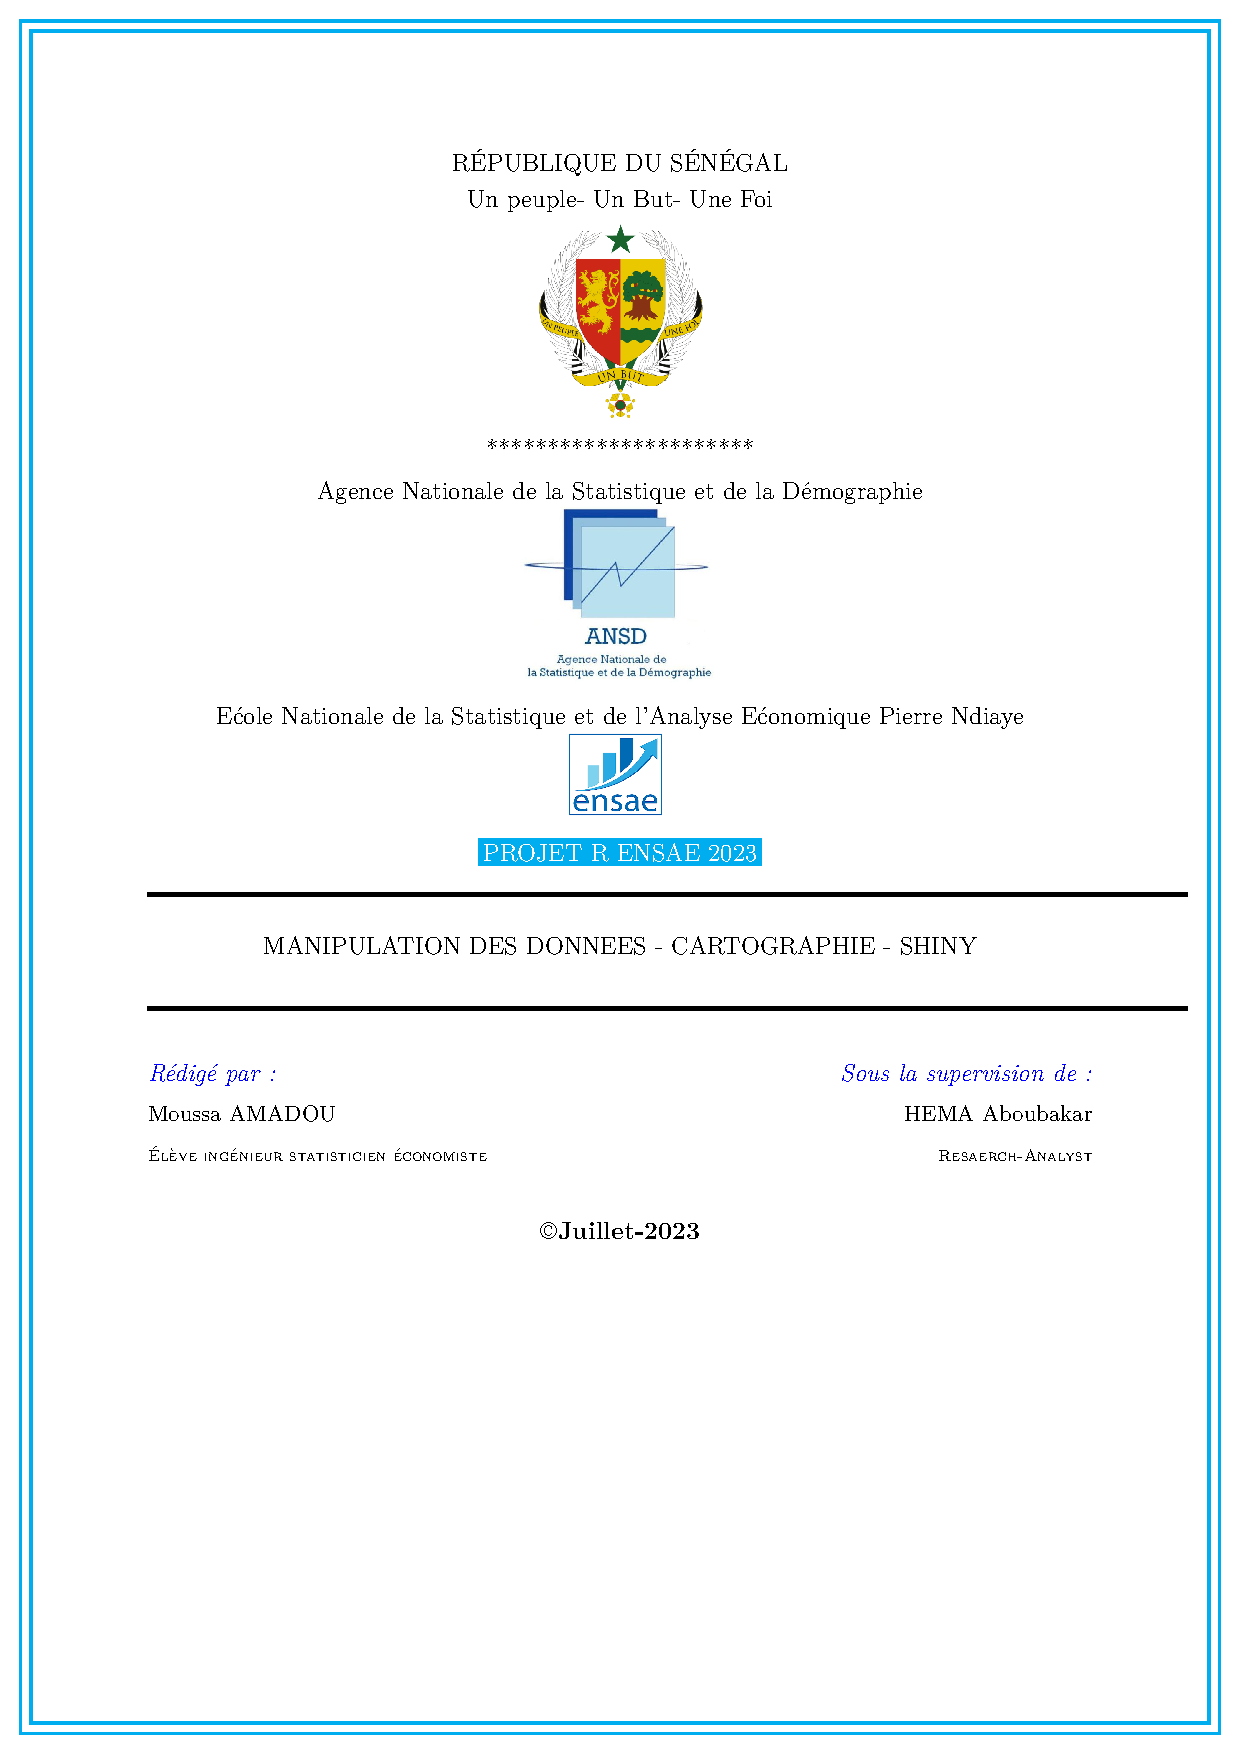
\includepdf{projet.pdf}

\renewcommand{\contentsname}{\textcolor{blue}{Table des matières}}

\textcolor{blue}{\tableofcontents}

\newpage

\hypertarget{introduction}{%
\section{INTRODUCTION}\label{introduction}}

Après avoir suivi 30 heures de cours intensifs sur le logiciel R,
encadrés par notre estimé maître, M. HEMA Aboubakar, analyste en
recherche, nous avons eu l'opportunité de nous immerger dans diverses
manipulations et fonctionnalités avancées de cet outil puissant. Ces
cours ont été enrichissants et nous ont permis de développer un large
éventail de compétences essentielles en analyse de données. Pendant
cette formation, nous avons abordé de nombreux sujets

passionnants, notamment :

\begin{itemize}
\tightlist
\item
  L'appurement et le traitement des données, où nous avons appris à
\end{itemize}

nettoyer et préparer des ensembles de données volumineux pour une

analyse précise.

\begin{itemize}
\tightlist
\item
  L'édition de documents sur R, en utilisant des techniques avancées
\end{itemize}

pour produire des rapports et des présentations de qualité

professionnelle.

\begin{itemize}
\tightlist
\item
  La cartographie, qui nous a permis de représenter graphiquement des
\end{itemize}

données spatiales et géographiques de manière visuellement attrayante.

\begin{itemize}
\tightlist
\item
  Rshiny, une plateforme qui nous a ouvert les portes à la création
\end{itemize}

d'applications interactives basées sur des analyses réalisées avec R.

\begin{itemize}
\tightlist
\item
  L'analyse de texte (textmining), une compétence puissante pour
\end{itemize}

extraire des informations significatives à partir de grandes quantités

de textes non structurés.

\begin{itemize}
\tightlist
\item
  Le calcul parallèle, nous permettant d'accélérer le traitement de
\end{itemize}

données massives en utilisant plusieurs cœurs de processeurs.

\begin{itemize}
\tightlist
\item
  L'intégration de Python dans R, combinant la puissance des deux
\end{itemize}

langages pour des analyses plus complexes.

\begin{itemize}
\tightlist
\item
  La résolution de systèmes d'équations linéaires, qui nous a aidés à
\end{itemize}

résoudre des problèmes mathématiques avancés.

\begin{itemize}
\tightlist
\item
  L'utilisation avancée des tableaux, pour une manipulation plus
\end{itemize}

efficace et une gestion optimale des données.

Tout au long de ce parcours d'apprentissage enrichissant, nous avons

développé des compétences solides qui nous permettront d'aborder des

projets de données complexes avec confiance et expertise.

Le projet final que nous entreprenons maintenant vise à mettre en

pratique l'ensemble des connaissances acquises lors de ce cours. Nous

sommes impatients de relever ce défi et de démontrer notre

compréhension approfondie du logiciel R. Grâce à cette expérience, nous
sommes convaincus que nous serons mieux préparés à relever les défis

analytiques du monde réel et à apporter des solutions innovantes aux

problèmes complexes auxquels nous serons confrontés dans notre domaine

de recherche.et de mettre en pratique les connaissances acquises en
classe

\newpage

\hypertarget{chargement-des-packages-importants}{%
\section{Chargement des packages
importants}\label{chargement-des-packages-importants}}

\begin{Shaded}
\begin{Highlighting}[]
\NormalTok{knitr}\SpecialCharTok{::}\NormalTok{opts\_chunk}\SpecialCharTok{$}\FunctionTok{set}\NormalTok{(}\AttributeTok{warning =} \ConstantTok{FALSE}\NormalTok{, }\AttributeTok{message =} \ConstantTok{FALSE}\NormalTok{)}
\FunctionTok{library}\NormalTok{(readxl) }\CommentTok{\# importer charger des données excel}
\FunctionTok{library}\NormalTok{(dplyr) }\CommentTok{\# pour la manipulation les bases de données}
\FunctionTok{library}\NormalTok{(gtsummary)}\CommentTok{\# pour les tableaux statistiques}
\FunctionTok{library}\NormalTok{(tidyverse)}\CommentTok{\# pour}
\FunctionTok{library}\NormalTok{(ggplot2) }\CommentTok{\# pour les graphiques}
\FunctionTok{library}\NormalTok{(ggridges)}\CommentTok{\# pour faire la courbe de densité}
\FunctionTok{library}\NormalTok{(huxtable) }\CommentTok{\# pour les tableaux }
\FunctionTok{library}\NormalTok{(fs) }\CommentTok{\# pour la cartographie}
\FunctionTok{library}\NormalTok{(gtsummary) }\CommentTok{\# tableaux avancés}
\FunctionTok{library}\NormalTok{(kableExtra) }\CommentTok{\# tableaux}
\FunctionTok{library}\NormalTok{(gridExtra) }\CommentTok{\# pour mettre deux tableaux cote à cote }
\FunctionTok{library}\NormalTok{(rgdal) }\CommentTok{\# mettre deux tableaux cote à cote}
\FunctionTok{library}\NormalTok{(stats) }\CommentTok{\# pour effectuer des tests statistiques }
\FunctionTok{library}\NormalTok{(devtools)}
\CommentTok{\#devtools:: install\_github("mikabr/ggpirate")}
\FunctionTok{library}\NormalTok{(ggplot2)}
\end{Highlighting}
\end{Shaded}

\newpage

\hypertarget{projet-1}{%
\section{PROJET 1}\label{projet-1}}

\hypertarget{importation-et-mise-en-forme}{%
\subsection{Importation et mise en
forme}\label{importation-et-mise-en-forme}}

\hypertarget{importation-de-la-base-de-donnuxe9es}{%
\subsection{\texorpdfstring{Importation de la base de données\\
}{Importation de la base de données }}\label{importation-de-la-base-de-donnuxe9es}}

\begin{Shaded}
\begin{Highlighting}[]
\CommentTok{\#\_\_\_\_\_\_\_\_\_\_\_\_\_\_\_\_\_\_\_\_\_\_on importe avec read\_xlsx\_\_\_\_\_\_\_\_\_\_\_\_\_\_\_\_\_\_\_\_\_\_\_\_\_\_\_\_\_\_\_}

\NormalTok{projet}\OtherTok{\textless{}{-}}\FunctionTok{read\_xlsx}\NormalTok{(}\StringTok{"Base\_Partie 1.xlsx"}\NormalTok{)  }
\end{Highlighting}
\end{Shaded}

\textbf{Il est necessaire de renommer les variables d'étude}\\

\begin{Shaded}
\begin{Highlighting}[]
\CommentTok{\#\_\_\_\_\_\_\_\_\_\_\_\_\_\_\_\_\_\_\_\_\_\_Renomer les variables\_\_\_\_\_\_\_\_\_\_\_\_\_\_\_\_\_\_\_\_\_\_\_\_\_\_\_\_\_\_\_\_}
\NormalTok{projet }\OtherTok{\textless{}{-}}\NormalTok{ projet }\SpecialCharTok{\%\textgreater{}\%} 
\NormalTok{  dplyr}\SpecialCharTok{::}\FunctionTok{rename}\NormalTok{(}\AttributeTok{Niveau\_instruction =}\NormalTok{ q25,}
                
                \AttributeTok{Statut\_juridique =}\NormalTok{ q12,}
                
                \AttributeTok{Proprietaire\_Locataire=}\NormalTok{q81,}
                       
                \AttributeTok{Activite\_principale=}\NormalTok{q8)}
\end{Highlighting}
\end{Shaded}

\hypertarget{tableau-qui-resume-les-valeurs-manquantes-par-variable}{%
\subsection{\texorpdfstring{Tableau qui resume les valeurs manquantes
par variable\\
}{Tableau qui resume les valeurs manquantes par variable }}\label{tableau-qui-resume-les-valeurs-manquantes-par-variable}}

\begin{Shaded}
\begin{Highlighting}[]
\CommentTok{\#\_\_\_\_\_\_\_\_\_Compter les valeurs manquantes pour chaque variable\_\_\_\_\_\_\_\_\_\_\_\_\_\_\_\_\_\_}

\NormalTok{missing\_counts }\OtherTok{\textless{}{-}}\NormalTok{ projet }\SpecialCharTok{\%\textgreater{}\%} 
  
\NormalTok{  dplyr}\SpecialCharTok{::} \FunctionTok{summarise}\NormalTok{(}\FunctionTok{across}\NormalTok{(}\FunctionTok{everything}\NormalTok{(), }
                           \SpecialCharTok{\textasciitilde{}}\FunctionTok{sum}\NormalTok{(}\FunctionTok{is.na}\NormalTok{(.))))}

\CommentTok{\#\_\_\_\_\_\_\_Convertir la table de comptage en format tbl\_summary\_\_\_\_\_\_\_\_\_\_\_\_\_\_\_\_\_\_\_}

\NormalTok{missing\_tbl }\OtherTok{\textless{}{-}}\NormalTok{ missing\_counts }\SpecialCharTok{\%\textgreater{}\%}
  \FunctionTok{pivot\_longer}\NormalTok{(}\FunctionTok{everything}\NormalTok{(), }
               \AttributeTok{names\_to =} \StringTok{"Variable"}\NormalTok{,}
               \AttributeTok{values\_to =} \StringTok{"Nbre observations manquantes"}\NormalTok{) }

\CommentTok{\#\_\_\_\_\_\_\_\_\_\_\_\_\_\_\_\_\_\_Afficher le tableau résultant\_\_\_\_\_\_\_\_\_\_\_\_\_\_\_\_\_\_\_\_\_\_\_\_\_\_\_\_\_\_\_}

\NormalTok{T1}\OtherTok{\textless{}{-}}\NormalTok{kableExtra}\SpecialCharTok{::}\FunctionTok{kable}\NormalTok{(}\FunctionTok{as.data.frame}\NormalTok{(missing\_tbl),}
                      \AttributeTok{caption =} \StringTok{"Nombre d\textquotesingle{}observations}
\StringTok{                      manquantes par variable"}\NormalTok{)}
\NormalTok{T1}
\end{Highlighting}
\end{Shaded}

\begin{table}

\caption{\label{tab:unnamed-chunk-4}Nombre d'observations
                      manquantes par variable}
\centering
\begin{tabular}[t]{l|r}
\hline
Variable & Nbre observations manquantes\\
\hline
key & 0\\
\hline
q1 & 0\\
\hline
q2 & 0\\
\hline
q23 & 0\\
\hline
q24 & 0\\
\hline
q24a\_1 & 0\\
\hline
q24a\_2 & 0\\
\hline
q24a\_3 & 0\\
\hline
q24a\_4 & 0\\
\hline
q24a\_5 & 0\\
\hline
q24a\_6 & 0\\
\hline
q24a\_7 & 0\\
\hline
q24a\_9 & 0\\
\hline
q24a\_10 & 0\\
\hline
Niveau\_instruction & 0\\
\hline
q26 & 0\\
\hline
Statut\_juridique & 0\\
\hline
q14b & 1\\
\hline
q16 & 1\\
\hline
q17 & 131\\
\hline
q19 & 120\\
\hline
q20 & 0\\
\hline
filiere\_1 & 0\\
\hline
filiere\_2 & 0\\
\hline
filiere\_3 & 0\\
\hline
filiere\_4 & 0\\
\hline
Activite\_principale & 0\\
\hline
Proprietaire\_Locataire & 0\\
\hline
gps\_menlatitude & 0\\
\hline
gps\_menlongitude & 0\\
\hline
submissiondate & 0\\
\hline
start & 0\\
\hline
today & 0\\
\hline
\end{tabular}
\end{table}

\newpage

\hypertarget{vuxe9rifions-sil-y-a-des-valeurs-manquantes-pour-la-variable-key}{%
\subsection{\texorpdfstring{\textbf{Vérifions s'il y a des valeurs
manquantes pour la variable~key}\\
}{Vérifions s'il y a des valeurs manquantes pour la variable~key }}\label{vuxe9rifions-sil-y-a-des-valeurs-manquantes-pour-la-variable-key}}

\begin{Shaded}
\begin{Highlighting}[]
\NormalTok{valeurs\_manquantes\_key }\OtherTok{\textless{}{-}} \FunctionTok{sum}\NormalTok{(}\FunctionTok{is.na}\NormalTok{(projet}\SpecialCharTok{$}\NormalTok{key))}

\CommentTok{\#\_\_\_\_\_\_\_\_\_\_\_\_\_Vérification et identification des PME concernées\_\_\_\_\_\_\_\_\_\_\_\_\_\_\_\_}

\ControlFlowTok{if}\NormalTok{ (valeurs\_manquantes\_key }\SpecialCharTok{\textgreater{}} \DecValTok{0}\NormalTok{) \{}
\NormalTok{  pme\_manquantes }\OtherTok{\textless{}{-}}\NormalTok{ projet}\SpecialCharTok{$}\NormalTok{nom\_de\_lacolonnedesPME[}\FunctionTok{which}\NormalTok{(}\FunctionTok{is.na}\NormalTok{(projet}\SpecialCharTok{$}\NormalTok{key))]}
  \FunctionTok{cat}\NormalTok{(}\StringTok{"Il y a"}\NormalTok{, }
\NormalTok{      valeurs\_manquantes\_key,}
      \StringTok{"valeurs manquantes pour la variable \textquotesingle{}key\textquotesingle{} dans la base de données du projet."}\NormalTok{)}
  \FunctionTok{cat}\NormalTok{(}\StringTok{"}\SpecialCharTok{\textbackslash{}n}\StringTok{Les PME concernées sont :"}\NormalTok{, }
      \FunctionTok{unique}\NormalTok{(pme\_manquantes))}
\NormalTok{\} }\ControlFlowTok{else}\NormalTok{ \{}
  \FunctionTok{cat}\NormalTok{(}\StringTok{"pas de valeurs manquantes pour la variable \textquotesingle{}key\textquotesingle{}."}\NormalTok{)}
\NormalTok{\}}
\end{Highlighting}
\end{Shaded}

\begin{verbatim}
## pas de valeurs manquantes pour la variable 'key'.
\end{verbatim}

\hypertarget{cruxe9ation-de-variables}{%
\subsection{\texorpdfstring{\textbf{Création de variables}\\
}{Création de variables }}\label{cruxe9ation-de-variables}}

\begin{Shaded}
\begin{Highlighting}[]
\NormalTok{projet }\OtherTok{\textless{}{-}}\NormalTok{ dplyr}\SpecialCharTok{::}\FunctionTok{rename}\NormalTok{(projet,}
                        \AttributeTok{region=}\NormalTok{q1,}
                        \AttributeTok{departement=}\NormalTok{q2,}
                        \AttributeTok{sexe=}\NormalTok{q23)}
\end{Highlighting}
\end{Shaded}

\hypertarget{cruxe9er-la-variable-sexe_2}{%
\subsection{\texorpdfstring{\textbf{Créer la variable sexe\_2}\\
}{Créer la variable sexe\_2 }}\label{cruxe9er-la-variable-sexe_2}}

\begin{Shaded}
\begin{Highlighting}[]
\CommentTok{\#\_\_\_\_\_\_\_\_\_\_\_\_\_\_\_\_\_\_\_\_\_\_\_\_\_initialisation\_\_\_\_\_\_\_\_\_\_\_\_\_\_\_\_\_\_\_\_\_\_\_\_\_\_\_\_\_\_\_\_\_\_\_\_\_\_\_}

\NormalTok{projet}\SpecialCharTok{$}\NormalTok{sexe\_2 }\OtherTok{\textless{}{-}} \DecValTok{0}

\CommentTok{\#\_\_\_\_\_\_\_\_\_\_\_\_\_\_\_\_\_\_\_\_\_\_\_\_\_affection des valeurs selon la condition\_\_\_\_\_\_\_\_\_\_\_\_}

\NormalTok{projet}\SpecialCharTok{$}\NormalTok{sexe\_2[projet}\SpecialCharTok{$}\NormalTok{sexe }\SpecialCharTok{==} \StringTok{"Femme"}\NormalTok{] }\OtherTok{\textless{}{-}} \DecValTok{1}
\end{Highlighting}
\end{Shaded}

\hypertarget{cruxe9er-un-data.frame-nommuxe9-langues}{%
\subsection{\texorpdfstring{\textbf{Créer un data.frame nommé langues}\\
}{Créer un data.frame nommé langues }}\label{cruxe9er-un-data.frame-nommuxe9-langues}}

\begin{Shaded}
\begin{Highlighting}[]
\CommentTok{\#\_\_\_\_\_\_\_\_\_\_\_\_\_\_\_\_\_\_ Variables communes\_\_\_\_\_\_\_\_\_\_\_\_\_\_\_\_\_\_\_\_\_\_\_\_\_\_\_\_\_\_\_\_\_}

\NormalTok{cle\_variable }\OtherTok{\textless{}{-}} \StringTok{"key"}
\CommentTok{\#\_\_\_\_\_\_\_\_\_\_\_\_\_\_\_\_\_\_\_\_\_\_\_\_\_\_\_\_\_\_\_\_\_\_\_\_\_\_\_\_\_\_\_\_\_\_\_\_\_\_\_\_\_\_\_\_\_\_\_\_\_\_\_\_\_\_\_\_\_\_\_}

\NormalTok{language\_variables }\OtherTok{\textless{}{-}} \FunctionTok{grep}\NormalTok{(}\StringTok{"\^{}q24a\_"}\NormalTok{,}
                           \FunctionTok{names}\NormalTok{(projet), }
                           \AttributeTok{value =} \ConstantTok{TRUE}\NormalTok{)}

\NormalTok{langues }\OtherTok{\textless{}{-}}\NormalTok{ projet[,}
                  \FunctionTok{c}\NormalTok{(cle\_variable, }
\NormalTok{                    language\_variables)]}

\CommentTok{\# Créer la variable "parle" égale au nombre de langues parlées}

\NormalTok{langues}\SpecialCharTok{$}\NormalTok{parle }\OtherTok{\textless{}{-}} \FunctionTok{rowSums}\NormalTok{(langues[, }
\NormalTok{                                 language\_variables])}

\CommentTok{\# Sélectionner uniquement les variables "key" et "parle" }

\NormalTok{langues }\OtherTok{\textless{}{-}}\NormalTok{ langues[, }
                   \FunctionTok{c}\NormalTok{(cle\_variable,}
                     \StringTok{"parle"}\NormalTok{)]}

\CommentTok{\# Fusionner les data.frames "projet" et "langues" en utilisant la variable "key"}

\NormalTok{projet }\OtherTok{\textless{}{-}} \FunctionTok{merge}\NormalTok{(projet, }
\NormalTok{                langues, }
                \AttributeTok{by =}\NormalTok{ cle\_variable)}
\end{Highlighting}
\end{Shaded}

\newpage

\hypertarget{analyses-descriptives}{%
\section{\texorpdfstring{\textbf{Analyses descriptives}\\
}{Analyses descriptives }}\label{analyses-descriptives}}

\hypertarget{detection-des-valeures-manquantes}{%
\subsection{\texorpdfstring{\textbf{Detection des valeures
manquantes}~}{Detection des valeures manquantes~}}\label{detection-des-valeures-manquantes}}

\begin{Shaded}
\begin{Highlighting}[]
\CommentTok{\# Filtrer les observations avec des valeurs aberrantes}

\NormalTok{projet\_aberrantes }\OtherTok{\textless{}{-}} \FunctionTok{subset}\NormalTok{(projet, }
\NormalTok{                            q24 }\SpecialCharTok{\textgreater{}}\DecValTok{99}\NormalTok{)}

\CommentTok{\# Créer un boxplot avec les valeurs aberrantes}

\FunctionTok{ggplot}\NormalTok{(projet\_aberrantes, }
       \FunctionTok{aes}\NormalTok{(}\AttributeTok{x =} \StringTok{""}\NormalTok{,}
           \AttributeTok{y =}\NormalTok{ q24)) }\SpecialCharTok{+}
  \FunctionTok{geom\_boxplot}\NormalTok{(}\AttributeTok{outlier.shape =}\ConstantTok{NA}\NormalTok{) }\SpecialCharTok{+} 
  
\CommentTok{\#Supprime les marqueurs par défaut des valeurs aberrantes}
  
  \FunctionTok{geom\_text}\NormalTok{(}\FunctionTok{aes}\NormalTok{(}\AttributeTok{label =}\NormalTok{ q24),}
            \AttributeTok{vjust =} \SpecialCharTok{{-}}\FloatTok{1.5}\NormalTok{) }\SpecialCharTok{+} 
  
\CommentTok{\#Affiche les valeurs numériques des valeurs aberrantes}
  
  \FunctionTok{labs}\NormalTok{(}\AttributeTok{title =} \StringTok{"Boxplot des Ages aberrants supérieures à 100 ans"}\NormalTok{,}
       \AttributeTok{x =} \StringTok{""}\NormalTok{,}
       \AttributeTok{y =} \StringTok{"AGE"}\NormalTok{)}
\end{Highlighting}
\end{Shaded}

\includegraphics{AMADOU_Moussa_files/figure-latex/unnamed-chunk-9-1.pdf}

\hypertarget{analyse-univariuxe9e-bivariuxe9e}{%
\subsection{\texorpdfstring{\textbf{Analyse univariée Bivariée}\\
}{Analyse univariée Bivariée }}\label{analyse-univariuxe9e-bivariuxe9e}}

\begin{Shaded}
\begin{Highlighting}[]
\NormalTok{tableau1 }\OtherTok{\textless{}{-}}\NormalTok{ projet }\SpecialCharTok{\%\textgreater{}\%} 
\NormalTok{  gtsummary}\SpecialCharTok{::}\FunctionTok{tbl\_summary}\NormalTok{(}
    \AttributeTok{include =} \FunctionTok{c}\NormalTok{(}\StringTok{"sexe"}\NormalTok{,}
                \StringTok{"Niveau\_instruction"}\NormalTok{,}
                \StringTok{"Statut\_juridique"}\NormalTok{,}
                \StringTok{"Proprietaire\_Locataire"}\NormalTok{),}
    \AttributeTok{statistic =} \FunctionTok{all\_categorical}\NormalTok{() }\SpecialCharTok{\textasciitilde{}} \StringTok{"\{p\} \% "}
\NormalTok{  ) }

\CommentTok{\# Analyse bivariée}

\NormalTok{tableau2 }\OtherTok{\textless{}{-}}\NormalTok{ projet }\SpecialCharTok{\%\textgreater{}\%} 
\NormalTok{  gtsummary}\SpecialCharTok{::}\FunctionTok{tbl\_summary}\NormalTok{(}
  \AttributeTok{include =} \FunctionTok{c}\NormalTok{(}\StringTok{"sexe"}\NormalTok{,}
              \StringTok{"Niveau\_instruction"}\NormalTok{,}
              \StringTok{"Statut\_juridique"}\NormalTok{,}
              \StringTok{"Proprietaire\_Locataire"}\NormalTok{),}
  \AttributeTok{by=}\StringTok{"sexe"}\NormalTok{,}
  \AttributeTok{statistic =} \FunctionTok{all\_categorical}\NormalTok{() }\SpecialCharTok{\textasciitilde{}} \StringTok{"\{p\} \% "}
\NormalTok{)}

\NormalTok{gtsummary}\SpecialCharTok{::} \FunctionTok{tbl\_merge}\NormalTok{(}
  \FunctionTok{list}\NormalTok{(tableau1, }
\NormalTok{       tableau2),}
  \AttributeTok{tab\_spanner =} \FunctionTok{c}\NormalTok{(}\StringTok{"**Analyse univariée**"}\NormalTok{,}
                  \StringTok{"**Analyse bivariée**"}\NormalTok{))}\SpecialCharTok{\%\textgreater{}\%}
  \FunctionTok{bold\_labels}\NormalTok{() }\SpecialCharTok{\%\textgreater{}\%}
  \FunctionTok{italicize\_levels}\NormalTok{() }\SpecialCharTok{\%\textgreater{}\%}  
  \FunctionTok{modify\_header}\NormalTok{(}
    \FunctionTok{list}\NormalTok{(}
\NormalTok{      label }\SpecialCharTok{\textasciitilde{}} \StringTok{"**Variables**"}\NormalTok{)}
\NormalTok{  )}\SpecialCharTok{\%\textgreater{}\%}
  \FunctionTok{add\_header\_above}\NormalTok{()}\SpecialCharTok{\%\textgreater{}\%}
 \FunctionTok{as\_gt}\NormalTok{() }
\end{Highlighting}
\end{Shaded}

\setlength{\LTpost}{0mm}
\begin{longtable}{lccc}
\toprule
 & \textbf{Analyse univariée} & \multicolumn{2}{c}{\textbf{Analyse bivariée}} \\ 
\cmidrule(lr){2-2} \cmidrule(lr){3-4}
\textbf{Variables} & \textbf{N = 250}\textsuperscript{\textit{1}} & \textbf{Femme}, N = 191\textsuperscript{\textit{1}} & \textbf{Homme}, N = 59\textsuperscript{\textit{1}} \\ 
\midrule
sexe &  &  &  \\ 
    Femme & 76 \%  &  &  \\ 
    Homme & 24 \%  &  &  \\ 
Niveau\_instruction &  &  &  \\ 
    Aucun niveau & 32 \%  & 37 \%  & 15 \%  \\ 
    Niveau primaire & 22 \%  & 25 \%  & 14 \%  \\ 
    Niveau secondaire & 30 \%  & 29 \%  & 31 \%  \\ 
    Niveau Superieur & 16 \%  & 8.9 \%  & 41 \%  \\ 
Statut\_juridique &  &  &  \\ 
    Association & 2.4 \%  & 1.6 \%  & 5.1 \%  \\ 
    GIE & 72 \%  & 78 \%  & 51 \%  \\ 
    Informel & 15 \%  & 17 \%  & 10 \%  \\ 
    SA & 2.8 \%  & 0.5 \%  & 10 \%  \\ 
    SARL & 5.2 \%  & 1.0 \%  & 19 \%  \\ 
    SUARL & 2.8 \%  & 2.1 \%  & 5.1 \%  \\ 
Proprietaire\_Locataire &  &  &  \\ 
    Locataire & 9.6 \%  & 8.4 \%  & 14 \%  \\ 
    Propriétaire & 90 \%  & 92 \%  & 86 \%  \\ 
\bottomrule
\end{longtable}
\begin{minipage}{\linewidth}
\textsuperscript{\textit{1}}\% \%\\
\end{minipage}

\newpage

\hypertarget{analyses-supplementaires}{%
\subsection{\texorpdfstring{\textbf{ANALYSES SUPPLEMENTAIRES}\\
}{ANALYSES SUPPLEMENTAIRES }}\label{analyses-supplementaires}}

\begin{Shaded}
\begin{Highlighting}[]
\CommentTok{\# Sélectionner les variables pour l\textquotesingle{}analyse par filière selon le sexe}

\NormalTok{tableau3 }\OtherTok{\textless{}{-}}\NormalTok{ projet }\SpecialCharTok{\%\textgreater{}\%}
  \FunctionTok{subset}\NormalTok{(filiere\_1 }\SpecialCharTok{==} \DecValTok{1}\NormalTok{) }\SpecialCharTok{\%\textgreater{}\%} 
\NormalTok{  gtsummary}\SpecialCharTok{::} \FunctionTok{tbl\_summary}\NormalTok{(}
    \AttributeTok{include =}\NormalTok{ region ,}
    \AttributeTok{by =}\NormalTok{ filiere\_1 ,}
    \AttributeTok{statistic =} \FunctionTok{all\_categorical}\NormalTok{() }\SpecialCharTok{\textasciitilde{}} \StringTok{"\{p\} \% "}\NormalTok{,}
    \AttributeTok{percent =} \StringTok{"col"}
\NormalTok{  ) }
\NormalTok{tableau4 }\OtherTok{\textless{}{-}}\NormalTok{ projet }\SpecialCharTok{\%\textgreater{}\%}
  \FunctionTok{subset}\NormalTok{(filiere\_2}\SpecialCharTok{==}\DecValTok{1}\NormalTok{) }\SpecialCharTok{\%\textgreater{}\%} 
\NormalTok{  gtsummary}\SpecialCharTok{::} \FunctionTok{tbl\_summary}\NormalTok{(}
    \AttributeTok{include =}\NormalTok{ region ,}
    \AttributeTok{by =}\NormalTok{ filiere\_2 ,}
    \AttributeTok{statistic =} \FunctionTok{all\_categorical}\NormalTok{() }\SpecialCharTok{\textasciitilde{}} \StringTok{"\{p\} \% "}\NormalTok{,}
    \AttributeTok{percent =} \StringTok{"col"}
\NormalTok{  ) }
\NormalTok{tableau5 }\OtherTok{\textless{}{-}}\NormalTok{ projet }\SpecialCharTok{\%\textgreater{}\%}
  \FunctionTok{subset}\NormalTok{(filiere\_3}\SpecialCharTok{==}\DecValTok{1}\NormalTok{) }\SpecialCharTok{\%\textgreater{}\%} 
\NormalTok{  gtsummary}\SpecialCharTok{::} \FunctionTok{tbl\_summary}\NormalTok{(}
    \AttributeTok{include =}\NormalTok{ region ,}
    \AttributeTok{by =}\NormalTok{ filiere\_3 ,}
    \AttributeTok{statistic =} \FunctionTok{all\_categorical}\NormalTok{() }\SpecialCharTok{\textasciitilde{}} \StringTok{"\{p\} \% "}\NormalTok{,}
    \AttributeTok{percent =} \StringTok{"col"}
\NormalTok{  ) }
\NormalTok{tableau6 }\OtherTok{\textless{}{-}}\NormalTok{ projet }\SpecialCharTok{\%\textgreater{}\%}
  \FunctionTok{subset}\NormalTok{(filiere\_4}\SpecialCharTok{==}\DecValTok{1}\NormalTok{) }\SpecialCharTok{\%\textgreater{}\%} 
\NormalTok{  gtsummary}\SpecialCharTok{::} \FunctionTok{tbl\_summary}\NormalTok{(}
    \AttributeTok{include =}\NormalTok{ region ,}
    \AttributeTok{by =}\NormalTok{ filiere\_4 ,}
    \AttributeTok{statistic =} \FunctionTok{all\_categorical}\NormalTok{() }\SpecialCharTok{\textasciitilde{}} \StringTok{"\{p\} \% "}\NormalTok{,}
    \AttributeTok{percent =} \StringTok{"col"}
\NormalTok{  ) }
\FunctionTok{tbl\_merge}\NormalTok{(}
  \FunctionTok{list}\NormalTok{(tableau3, tableau4,tableau5,tableau6),}
  \AttributeTok{tab\_spanner =} \FunctionTok{c}\NormalTok{(}\StringTok{"**FILIERE ARACHIDE**"}\NormalTok{, }
                  \StringTok{"**FILIERE ANACARDE**"}\NormalTok{,}
                  \StringTok{"**FILIERE MANGUE**"}\NormalTok{,}
                  \StringTok{"**FILIERE RIZ**"}\NormalTok{))}\SpecialCharTok{\%\textgreater{}\%}
  \FunctionTok{bold\_labels}\NormalTok{() }\SpecialCharTok{\%\textgreater{}\%}
  \FunctionTok{italicize\_levels}\NormalTok{() }\SpecialCharTok{\%\textgreater{}\%}  
  \FunctionTok{modify\_header}\NormalTok{(}
    \FunctionTok{list}\NormalTok{(}
\NormalTok{      label }\SpecialCharTok{\textasciitilde{}} \StringTok{"**PRODUCTION**"}\NormalTok{)}
\NormalTok{  )}\SpecialCharTok{\%\textgreater{}\%}
  \FunctionTok{add\_header\_above}\NormalTok{() }\SpecialCharTok{\%\textgreater{}\%} 
  \FunctionTok{as\_hux\_table}\NormalTok{()}\CommentTok{\# transformer le tableau }
\end{Highlighting}
\end{Shaded}

 
  \providecommand{\huxb}[2]{\arrayrulecolor[RGB]{#1}\global\arrayrulewidth=#2pt}
  \providecommand{\huxvb}[2]{\color[RGB]{#1}\vrule width #2pt}
  \providecommand{\huxtpad}[1]{\rule{0pt}{#1}}
  \providecommand{\huxbpad}[1]{\rule[-#1]{0pt}{#1}}

\begin{table}[ht]
\begin{centerbox}
\begin{threeparttable}
 \label{tab:unnamed-chunk-11}
\setlength{\tabcolsep}{0pt}
\begin{tabular}{l l l l l}


\hhline{}
\arrayrulecolor{black}

\multicolumn{1}{!{\huxvb{0, 0, 0}{0}}l!{\huxvb{0, 0, 0}{0}}}{\huxtpad{6pt + 1em}\raggedright \hspace{6pt} 
 \hspace{6pt}\huxbpad{6pt}} &
\multicolumn{1}{c!{\huxvb{0, 0, 0}{0}}}{\huxtpad{6pt + 1em}\centering \hspace{6pt} \textbf{FILIERE ARACHIDE}
 \hspace{6pt}\huxbpad{6pt}} &
\multicolumn{1}{c!{\huxvb{0, 0, 0}{0}}}{\huxtpad{6pt + 1em}\centering \hspace{6pt} \textbf{FILIERE ANACARDE}
 \hspace{6pt}\huxbpad{6pt}} &
\multicolumn{1}{c!{\huxvb{0, 0, 0}{0}}}{\huxtpad{6pt + 1em}\centering \hspace{6pt} \textbf{FILIERE MANGUE}
 \hspace{6pt}\huxbpad{6pt}} &
\multicolumn{1}{c!{\huxvb{0, 0, 0}{0}}}{\huxtpad{6pt + 1em}\centering \hspace{6pt} \textbf{FILIERE RIZ}
 \hspace{6pt}\huxbpad{6pt}} \tabularnewline[-0.5pt]


\hhline{}
\arrayrulecolor{black}

\multicolumn{1}{!{\huxvb{0, 0, 0}{0}}l!{\huxvb{0, 0, 0}{0}}}{\huxtpad{6pt + 1em}\raggedright \hspace{6pt} \textbf{PRODUCTION}
 \hspace{6pt}\huxbpad{6pt}} &
\multicolumn{1}{c!{\huxvb{0, 0, 0}{0}}}{\huxtpad{6pt + 1em}\centering \hspace{6pt} \textbf{1}, N = 108
 \hspace{6pt}\huxbpad{6pt}} &
\multicolumn{1}{c!{\huxvb{0, 0, 0}{0}}}{\huxtpad{6pt + 1em}\centering \hspace{6pt} \textbf{1}, N = 61
 \hspace{6pt}\huxbpad{6pt}} &
\multicolumn{1}{c!{\huxvb{0, 0, 0}{0}}}{\huxtpad{6pt + 1em}\centering \hspace{6pt} \textbf{1}, N = 89
 \hspace{6pt}\huxbpad{6pt}} &
\multicolumn{1}{c!{\huxvb{0, 0, 0}{0}}}{\huxtpad{6pt + 1em}\centering \hspace{6pt} \textbf{1}, N = 92
 \hspace{6pt}\huxbpad{6pt}} \tabularnewline[-0.5pt]


\hhline{>{\huxb{0, 0, 0}{0.4}}->{\huxb{0, 0, 0}{0.4}}->{\huxb{0, 0, 0}{0.4}}->{\huxb{0, 0, 0}{0.4}}->{\huxb{0, 0, 0}{0.4}}-}
\arrayrulecolor{black}

\multicolumn{1}{!{\huxvb{0, 0, 0}{0}}l!{\huxvb{0, 0, 0}{0}}}{\huxtpad{6pt + 1em}\raggedright \hspace{6pt} \textbf{region} \hspace{6pt}\huxbpad{6pt}} &
\multicolumn{1}{c!{\huxvb{0, 0, 0}{0}}}{\huxtpad{6pt + 1em}\centering \hspace{6pt}  \hspace{6pt}\huxbpad{6pt}} &
\multicolumn{1}{c!{\huxvb{0, 0, 0}{0}}}{\huxtpad{6pt + 1em}\centering \hspace{6pt}  \hspace{6pt}\huxbpad{6pt}} &
\multicolumn{1}{c!{\huxvb{0, 0, 0}{0}}}{\huxtpad{6pt + 1em}\centering \hspace{6pt}  \hspace{6pt}\huxbpad{6pt}} &
\multicolumn{1}{c!{\huxvb{0, 0, 0}{0}}}{\huxtpad{6pt + 1em}\centering \hspace{6pt}  \hspace{6pt}\huxbpad{6pt}} \tabularnewline[-0.5pt]


\hhline{}
\arrayrulecolor{black}

\multicolumn{1}{!{\huxvb{0, 0, 0}{0}}l!{\huxvb{0, 0, 0}{0}}}{\huxtpad{6pt + 1em}\raggedright \hspace{15pt} \textit{Diourbel} \hspace{6pt}\huxbpad{6pt}} &
\multicolumn{1}{c!{\huxvb{0, 0, 0}{0}}}{\huxtpad{6pt + 1em}\centering \hspace{6pt} 31 \%  \hspace{6pt}\huxbpad{6pt}} &
\multicolumn{1}{c!{\huxvb{0, 0, 0}{0}}}{\huxtpad{6pt + 1em}\centering \hspace{6pt}  \hspace{6pt}\huxbpad{6pt}} &
\multicolumn{1}{c!{\huxvb{0, 0, 0}{0}}}{\huxtpad{6pt + 1em}\centering \hspace{6pt} 1.1 \%  \hspace{6pt}\huxbpad{6pt}} &
\multicolumn{1}{c!{\huxvb{0, 0, 0}{0}}}{\huxtpad{6pt + 1em}\centering \hspace{6pt}  \hspace{6pt}\huxbpad{6pt}} \tabularnewline[-0.5pt]


\hhline{}
\arrayrulecolor{black}

\multicolumn{1}{!{\huxvb{0, 0, 0}{0}}l!{\huxvb{0, 0, 0}{0}}}{\huxtpad{6pt + 1em}\raggedright \hspace{15pt} \textit{Fatick} \hspace{6pt}\huxbpad{6pt}} &
\multicolumn{1}{c!{\huxvb{0, 0, 0}{0}}}{\huxtpad{6pt + 1em}\centering \hspace{6pt} 11 \%  \hspace{6pt}\huxbpad{6pt}} &
\multicolumn{1}{c!{\huxvb{0, 0, 0}{0}}}{\huxtpad{6pt + 1em}\centering \hspace{6pt} 34 \%  \hspace{6pt}\huxbpad{6pt}} &
\multicolumn{1}{c!{\huxvb{0, 0, 0}{0}}}{\huxtpad{6pt + 1em}\centering \hspace{6pt} 3.4 \%  \hspace{6pt}\huxbpad{6pt}} &
\multicolumn{1}{c!{\huxvb{0, 0, 0}{0}}}{\huxtpad{6pt + 1em}\centering \hspace{6pt} 4.3 \%  \hspace{6pt}\huxbpad{6pt}} \tabularnewline[-0.5pt]


\hhline{}
\arrayrulecolor{black}

\multicolumn{1}{!{\huxvb{0, 0, 0}{0}}l!{\huxvb{0, 0, 0}{0}}}{\huxtpad{6pt + 1em}\raggedright \hspace{15pt} \textit{Kaffrine} \hspace{6pt}\huxbpad{6pt}} &
\multicolumn{1}{c!{\huxvb{0, 0, 0}{0}}}{\huxtpad{6pt + 1em}\centering \hspace{6pt} 7.4 \%  \hspace{6pt}\huxbpad{6pt}} &
\multicolumn{1}{c!{\huxvb{0, 0, 0}{0}}}{\huxtpad{6pt + 1em}\centering \hspace{6pt}  \hspace{6pt}\huxbpad{6pt}} &
\multicolumn{1}{c!{\huxvb{0, 0, 0}{0}}}{\huxtpad{6pt + 1em}\centering \hspace{6pt} 5.6 \%  \hspace{6pt}\huxbpad{6pt}} &
\multicolumn{1}{c!{\huxvb{0, 0, 0}{0}}}{\huxtpad{6pt + 1em}\centering \hspace{6pt} 1.1 \%  \hspace{6pt}\huxbpad{6pt}} \tabularnewline[-0.5pt]


\hhline{}
\arrayrulecolor{black}

\multicolumn{1}{!{\huxvb{0, 0, 0}{0}}l!{\huxvb{0, 0, 0}{0}}}{\huxtpad{6pt + 1em}\raggedright \hspace{15pt} \textit{Kaolack} \hspace{6pt}\huxbpad{6pt}} &
\multicolumn{1}{c!{\huxvb{0, 0, 0}{0}}}{\huxtpad{6pt + 1em}\centering \hspace{6pt} 19 \%  \hspace{6pt}\huxbpad{6pt}} &
\multicolumn{1}{c!{\huxvb{0, 0, 0}{0}}}{\huxtpad{6pt + 1em}\centering \hspace{6pt}  \hspace{6pt}\huxbpad{6pt}} &
\multicolumn{1}{c!{\huxvb{0, 0, 0}{0}}}{\huxtpad{6pt + 1em}\centering \hspace{6pt} 7.9 \%  \hspace{6pt}\huxbpad{6pt}} &
\multicolumn{1}{c!{\huxvb{0, 0, 0}{0}}}{\huxtpad{6pt + 1em}\centering \hspace{6pt} 4.3 \%  \hspace{6pt}\huxbpad{6pt}} \tabularnewline[-0.5pt]


\hhline{}
\arrayrulecolor{black}

\multicolumn{1}{!{\huxvb{0, 0, 0}{0}}l!{\huxvb{0, 0, 0}{0}}}{\huxtpad{6pt + 1em}\raggedright \hspace{15pt} \textit{Kolda} \hspace{6pt}\huxbpad{6pt}} &
\multicolumn{1}{c!{\huxvb{0, 0, 0}{0}}}{\huxtpad{6pt + 1em}\centering \hspace{6pt} 0.9 \%  \hspace{6pt}\huxbpad{6pt}} &
\multicolumn{1}{c!{\huxvb{0, 0, 0}{0}}}{\huxtpad{6pt + 1em}\centering \hspace{6pt} 8.2 \%  \hspace{6pt}\huxbpad{6pt}} &
\multicolumn{1}{c!{\huxvb{0, 0, 0}{0}}}{\huxtpad{6pt + 1em}\centering \hspace{6pt}  \hspace{6pt}\huxbpad{6pt}} &
\multicolumn{1}{c!{\huxvb{0, 0, 0}{0}}}{\huxtpad{6pt + 1em}\centering \hspace{6pt} 4.3 \%  \hspace{6pt}\huxbpad{6pt}} \tabularnewline[-0.5pt]


\hhline{}
\arrayrulecolor{black}

\multicolumn{1}{!{\huxvb{0, 0, 0}{0}}l!{\huxvb{0, 0, 0}{0}}}{\huxtpad{6pt + 1em}\raggedright \hspace{15pt} \textit{Saint-Louis} \hspace{6pt}\huxbpad{6pt}} &
\multicolumn{1}{c!{\huxvb{0, 0, 0}{0}}}{\huxtpad{6pt + 1em}\centering \hspace{6pt} 0.9 \%  \hspace{6pt}\huxbpad{6pt}} &
\multicolumn{1}{c!{\huxvb{0, 0, 0}{0}}}{\huxtpad{6pt + 1em}\centering \hspace{6pt}  \hspace{6pt}\huxbpad{6pt}} &
\multicolumn{1}{c!{\huxvb{0, 0, 0}{0}}}{\huxtpad{6pt + 1em}\centering \hspace{6pt} 47 \%  \hspace{6pt}\huxbpad{6pt}} &
\multicolumn{1}{c!{\huxvb{0, 0, 0}{0}}}{\huxtpad{6pt + 1em}\centering \hspace{6pt}  \hspace{6pt}\huxbpad{6pt}} \tabularnewline[-0.5pt]


\hhline{}
\arrayrulecolor{black}

\multicolumn{1}{!{\huxvb{0, 0, 0}{0}}l!{\huxvb{0, 0, 0}{0}}}{\huxtpad{6pt + 1em}\raggedright \hspace{15pt} \textit{Thiès} \hspace{6pt}\huxbpad{6pt}} &
\multicolumn{1}{c!{\huxvb{0, 0, 0}{0}}}{\huxtpad{6pt + 1em}\centering \hspace{6pt} 25 \%  \hspace{6pt}\huxbpad{6pt}} &
\multicolumn{1}{c!{\huxvb{0, 0, 0}{0}}}{\huxtpad{6pt + 1em}\centering \hspace{6pt}  \hspace{6pt}\huxbpad{6pt}} &
\multicolumn{1}{c!{\huxvb{0, 0, 0}{0}}}{\huxtpad{6pt + 1em}\centering \hspace{6pt} 28 \%  \hspace{6pt}\huxbpad{6pt}} &
\multicolumn{1}{c!{\huxvb{0, 0, 0}{0}}}{\huxtpad{6pt + 1em}\centering \hspace{6pt} 35 \%  \hspace{6pt}\huxbpad{6pt}} \tabularnewline[-0.5pt]


\hhline{}
\arrayrulecolor{black}

\multicolumn{1}{!{\huxvb{0, 0, 0}{0}}l!{\huxvb{0, 0, 0}{0}}}{\huxtpad{6pt + 1em}\raggedright \hspace{15pt} \textit{Ziguinchor} \hspace{6pt}\huxbpad{6pt}} &
\multicolumn{1}{c!{\huxvb{0, 0, 0}{0}}}{\huxtpad{6pt + 1em}\centering \hspace{6pt} 5.6 \%  \hspace{6pt}\huxbpad{6pt}} &
\multicolumn{1}{c!{\huxvb{0, 0, 0}{0}}}{\huxtpad{6pt + 1em}\centering \hspace{6pt} 51 \%  \hspace{6pt}\huxbpad{6pt}} &
\multicolumn{1}{c!{\huxvb{0, 0, 0}{0}}}{\huxtpad{6pt + 1em}\centering \hspace{6pt} 6.7 \%  \hspace{6pt}\huxbpad{6pt}} &
\multicolumn{1}{c!{\huxvb{0, 0, 0}{0}}}{\huxtpad{6pt + 1em}\centering \hspace{6pt} 47 \%  \hspace{6pt}\huxbpad{6pt}} \tabularnewline[-0.5pt]


\hhline{}
\arrayrulecolor{black}

\multicolumn{1}{!{\huxvb{0, 0, 0}{0}}l!{\huxvb{0, 0, 0}{0}}}{\huxtpad{6pt + 1em}\raggedright \hspace{15pt} \textit{Dakar} \hspace{6pt}\huxbpad{6pt}} &
\multicolumn{1}{c!{\huxvb{0, 0, 0}{0}}}{\huxtpad{6pt + 1em}\centering \hspace{6pt}  \hspace{6pt}\huxbpad{6pt}} &
\multicolumn{1}{c!{\huxvb{0, 0, 0}{0}}}{\huxtpad{6pt + 1em}\centering \hspace{6pt} 1.6 \%  \hspace{6pt}\huxbpad{6pt}} &
\multicolumn{1}{c!{\huxvb{0, 0, 0}{0}}}{\huxtpad{6pt + 1em}\centering \hspace{6pt}  \hspace{6pt}\huxbpad{6pt}} &
\multicolumn{1}{c!{\huxvb{0, 0, 0}{0}}}{\huxtpad{6pt + 1em}\centering \hspace{6pt} 1.1 \%  \hspace{6pt}\huxbpad{6pt}} \tabularnewline[-0.5pt]


\hhline{}
\arrayrulecolor{black}

\multicolumn{1}{!{\huxvb{0, 0, 0}{0}}l!{\huxvb{0, 0, 0}{0}}}{\huxtpad{6pt + 1em}\raggedright \hspace{15pt} \textit{Sédhiou} \hspace{6pt}\huxbpad{6pt}} &
\multicolumn{1}{c!{\huxvb{0, 0, 0}{0}}}{\huxtpad{6pt + 1em}\centering \hspace{6pt}  \hspace{6pt}\huxbpad{6pt}} &
\multicolumn{1}{c!{\huxvb{0, 0, 0}{0}}}{\huxtpad{6pt + 1em}\centering \hspace{6pt} 4.9 \%  \hspace{6pt}\huxbpad{6pt}} &
\multicolumn{1}{c!{\huxvb{0, 0, 0}{0}}}{\huxtpad{6pt + 1em}\centering \hspace{6pt}  \hspace{6pt}\huxbpad{6pt}} &
\multicolumn{1}{c!{\huxvb{0, 0, 0}{0}}}{\huxtpad{6pt + 1em}\centering \hspace{6pt} 3.3 \%  \hspace{6pt}\huxbpad{6pt}} \tabularnewline[-0.5pt]


\hhline{>{\huxb{0, 0, 0}{0.8}}->{\huxb{0, 0, 0}{0.8}}->{\huxb{0, 0, 0}{0.8}}->{\huxb{0, 0, 0}{0.8}}->{\huxb{0, 0, 0}{0.8}}-}
\arrayrulecolor{black}

\multicolumn{5}{!{\huxvb{0, 0, 0}{0}}l!{\huxvb{0, 0, 0}{0}}}{\huxtpad{6pt + 1em}\raggedright \hspace{6pt} \% \%  \hspace{6pt}\huxbpad{6pt}} \tabularnewline[-0.5pt]


\hhline{}
\arrayrulecolor{black}
\end{tabular}
\end{threeparttable}\par\end{centerbox}

\end{table}
 

\newpage

\hypertarget{representation}{%
\subsubsection{\texorpdfstring{\textbf{Representation}~}{Representation~}}\label{representation}}

\begin{Shaded}
\begin{Highlighting}[]
\FunctionTok{ggplot}\NormalTok{(projet, }
       \FunctionTok{aes}\NormalTok{(}\AttributeTok{x =}\NormalTok{ Niveau\_instruction,}
                   \AttributeTok{fill =}\NormalTok{ Statut\_juridique))}\SpecialCharTok{+}
 \FunctionTok{geom\_bar}\NormalTok{(}\AttributeTok{position =} \StringTok{"dodge"}\NormalTok{, }
          \AttributeTok{stat =} \StringTok{"count"}\NormalTok{)}\SpecialCharTok{+}
  \FunctionTok{labs}\NormalTok{(}\AttributeTok{title =} \StringTok{"Niveau\_instruction selon Statut\_juridique"}\NormalTok{)}\SpecialCharTok{+}
 \FunctionTok{theme\_classic}\NormalTok{() }
\end{Highlighting}
\end{Shaded}

\includegraphics{AMADOU_Moussa_files/figure-latex/unnamed-chunk-12-1.pdf}

\newpage

\hypertarget{courbes-de-densituxe9}{%
\subsection{\texorpdfstring{\textbf{Courbes de densité}\\
}{Courbes de densité }}\label{courbes-de-densituxe9}}

\begin{Shaded}
\begin{Highlighting}[]
\FunctionTok{ggplot}\NormalTok{(projet, }\FunctionTok{aes}\NormalTok{(}\AttributeTok{x =}\NormalTok{ sexe,}
                   \AttributeTok{y =}\NormalTok{ Activite\_principale)) }\SpecialCharTok{+}
  
  \FunctionTok{geom\_density\_ridges}\NormalTok{(}\FunctionTok{aes}\NormalTok{(}\AttributeTok{fill =}\NormalTok{  Activite\_principale)) }\SpecialCharTok{+}
  
  \FunctionTok{scale\_fill\_manual}\NormalTok{(}\AttributeTok{values =} \FunctionTok{c}\NormalTok{(}\StringTok{"\#00AFBB"}\NormalTok{,}
                               \StringTok{"\#E7B800"}\NormalTok{, }
                               \StringTok{"\#FC4E07"}\NormalTok{,}
                               \StringTok{"\#FC4E07"}\NormalTok{,}
                               \StringTok{"\#00AFBB"}\NormalTok{,}
                               \StringTok{"\#FC4E07"}\NormalTok{,}
                               \StringTok{"\#E7B800"}\NormalTok{,}
                               \StringTok{"\#00AFBB"}\NormalTok{,}
                               \StringTok{"\#FC4E07"}\NormalTok{))}\SpecialCharTok{+}
  
  \FunctionTok{labs}\NormalTok{(}\AttributeTok{title =} \StringTok{"Courbe de densité"}\NormalTok{)}
\end{Highlighting}
\end{Shaded}

\includegraphics{AMADOU_Moussa_files/figure-latex/unnamed-chunk-13-1.pdf}

\newpage

\begin{Shaded}
\begin{Highlighting}[]
\CommentTok{\# Chargement des bibliothèques nécessaires}
\FunctionTok{library}\NormalTok{(ggplot2)}
\FunctionTok{library}\NormalTok{(ggpirate)}
\FunctionTok{library}\NormalTok{(gridExtra)}

\CommentTok{\# Répartition 1 : Filtrer les données et renommer la variable "q24" en "age"}
\NormalTok{Repartition1 }\OtherTok{\textless{}{-}}\NormalTok{ projet }\SpecialCharTok{\%\textgreater{}\%}
  \FunctionTok{rename}\NormalTok{(}\AttributeTok{age =}\NormalTok{ q24) }\SpecialCharTok{\%\textgreater{}\%}
  \FunctionTok{filter}\NormalTok{(age }\SpecialCharTok{\textless{}} \DecValTok{120}\NormalTok{)}

\CommentTok{\# Répartition 2 : Filtrer les données et renommer la variable "q26" en "Annees\_experience"}
\NormalTok{Repartition2 }\OtherTok{\textless{}{-}}\NormalTok{ projet }\SpecialCharTok{\%\textgreater{}\%}
  \FunctionTok{rename}\NormalTok{(}\AttributeTok{Annees\_experience =}\NormalTok{ q26) }\SpecialCharTok{\%\textgreater{}\%}
  \FunctionTok{filter}\NormalTok{(Annees\_experience }\SpecialCharTok{\textless{}} \DecValTok{50}\NormalTok{)}

\CommentTok{\# Création du premier graphique (Répartition par âge selon le sexe)}
\NormalTok{plot1 }\OtherTok{\textless{}{-}} \FunctionTok{ggplot}\NormalTok{(Repartition1, }\FunctionTok{aes}\NormalTok{(}\AttributeTok{x =}\NormalTok{ sexe, }\AttributeTok{y =}\NormalTok{ age)) }\SpecialCharTok{+}
  \FunctionTok{geom\_pirate}\NormalTok{(}\FunctionTok{aes}\NormalTok{(}\AttributeTok{colour =}\NormalTok{ sexe)) }\SpecialCharTok{+}
  \FunctionTok{xlab}\NormalTok{(}\StringTok{"Sexe"}\NormalTok{) }\SpecialCharTok{+}
  \FunctionTok{ylab}\NormalTok{(}\StringTok{"Âge"}\NormalTok{) }\SpecialCharTok{+}
  \FunctionTok{ggtitle}\NormalTok{(}\StringTok{"Répartition par âge selon le sexe"}\NormalTok{) }\SpecialCharTok{+}
  \FunctionTok{theme\_light}\NormalTok{() }\SpecialCharTok{+}
  \FunctionTok{theme}\NormalTok{(}\AttributeTok{plot.title =} \FunctionTok{element\_text}\NormalTok{(}\AttributeTok{color =} \StringTok{"blue"}\NormalTok{))}

\CommentTok{\# Création du deuxième graphique (Années d\textquotesingle{}expérience selon le sexe)}
\NormalTok{plot2 }\OtherTok{\textless{}{-}} \FunctionTok{ggplot}\NormalTok{(Repartition2, }\FunctionTok{aes}\NormalTok{(}\AttributeTok{x =}\NormalTok{ sexe, }\AttributeTok{y =}\NormalTok{ Annees\_experience)) }\SpecialCharTok{+}
  \FunctionTok{geom\_pirate}\NormalTok{(}\FunctionTok{aes}\NormalTok{(}\AttributeTok{colour =}\NormalTok{ sexe)) }\SpecialCharTok{+}
  \FunctionTok{xlab}\NormalTok{(}\StringTok{"Sexe"}\NormalTok{) }\SpecialCharTok{+}
  \FunctionTok{ylab}\NormalTok{(}\StringTok{"Nombre d\textquotesingle{}années d\textquotesingle{}expérience"}\NormalTok{) }\SpecialCharTok{+}
  \FunctionTok{ggtitle}\NormalTok{(}\StringTok{"Années d\textquotesingle{}expérience selon le sexe"}\NormalTok{) }\SpecialCharTok{+}
  \FunctionTok{theme\_light}\NormalTok{() }\SpecialCharTok{+}
  \FunctionTok{theme}\NormalTok{(}\AttributeTok{plot.title =} \FunctionTok{element\_text}\NormalTok{(}\AttributeTok{color =} \StringTok{"blue"}\NormalTok{))}

\CommentTok{\# Afficher les graphiques côte à côte sur une même ligne}
\FunctionTok{grid.arrange}\NormalTok{(plot1, plot2, }\AttributeTok{ncol =} \DecValTok{2}\NormalTok{)}
\end{Highlighting}
\end{Shaded}

\includegraphics{AMADOU_Moussa_files/figure-latex/unnamed-chunk-14-1.pdf}

\hypertarget{visualisation-des-donnuxe9es-temporelles}{%
\subsection{\texorpdfstring{\textbf{Visualisation des données
temporelles}\\
}{Visualisation des données temporelles }}\label{visualisation-des-donnuxe9es-temporelles}}

\begin{Shaded}
\begin{Highlighting}[]
\FunctionTok{ggplot}\NormalTok{(projet, }
       \FunctionTok{aes}\NormalTok{(}\AttributeTok{x=}\NormalTok{start,}
           \AttributeTok{y=}\NormalTok{submissiondate))}\SpecialCharTok{+}
  
    \FunctionTok{geom\_line}\NormalTok{()}\SpecialCharTok{+} 
  
  \FunctionTok{theme}\NormalTok{(}\AttributeTok{plot.title =} \FunctionTok{element\_text}\NormalTok{(}\AttributeTok{hjust =} \FloatTok{0.1}\NormalTok{)) }\SpecialCharTok{+} 
  
  \FunctionTok{theme}\NormalTok{(}\AttributeTok{plot.background =} \FunctionTok{element\_rect}\NormalTok{(}\AttributeTok{fill =} \StringTok{"green"}\NormalTok{,}
                                       
                                       \AttributeTok{colour =} \StringTok{"black"}\NormalTok{)) }\SpecialCharTok{+} 
  
  \FunctionTok{theme}\NormalTok{(}\AttributeTok{panel.background =} \FunctionTok{element\_rect}\NormalTok{(}\AttributeTok{fill =} \StringTok{"white"}\NormalTok{,}
                                        
                                        \AttributeTok{colour =} \StringTok{"black"}\NormalTok{)) }\SpecialCharTok{+} 
  
  \FunctionTok{theme}\NormalTok{(}\AttributeTok{panel.grid.major =} \FunctionTok{element\_line}\NormalTok{(}\AttributeTok{colour =} \StringTok{"gray"}\NormalTok{, }
                                        
                                        \AttributeTok{linetype =} \StringTok{"dashed"}\NormalTok{))}\SpecialCharTok{+}
  
  \FunctionTok{labs}\NormalTok{(}\AttributeTok{title =} \StringTok{"Debut de l\textquotesingle{}interview par jour"}\NormalTok{,}
       
       \AttributeTok{x =} \StringTok{" DEBUT"}\NormalTok{,}
       
       \AttributeTok{y =} \StringTok{"Soumission"}\NormalTok{)}
\end{Highlighting}
\end{Shaded}

\includegraphics{AMADOU_Moussa_files/figure-latex/unnamed-chunk-15-1.pdf}

\newpage

\hypertarget{cartographie}{%
\section{\texorpdfstring{Cartographie\\
}{Cartographie }}\label{cartographie}}

\hypertarget{transformer-le-data.frame-en-donnuxe9es-guxe9ographiques-dont-lobjet-sera-nommuxe9-projet_map.}{%
\subsection{\texorpdfstring{\textbf{Transformer le data.frame en données
géographiques dont l'objet sera nommé projet\_map.}\\
}{Transformer le data.frame en données géographiques dont l'objet sera nommé projet\_map. }}\label{transformer-le-data.frame-en-donnuxe9es-guxe9ographiques-dont-lobjet-sera-nommuxe9-projet_map.}}

\begin{Shaded}
\begin{Highlighting}[]
\FunctionTok{library}\NormalTok{(sf)}

\CommentTok{\# chargement des données du senegal gadm}

\NormalTok{sen\_sf }\OtherTok{\textless{}{-}} \FunctionTok{st\_read}\NormalTok{(}\StringTok{"données\_SEN/gadm36\_SEN\_1.shp"}\NormalTok{)}
\end{Highlighting}
\end{Shaded}

\begin{verbatim}
## Reading layer `gadm36_SEN_1' from data source 
##   `C:\Users\USER\Documents\Projet_R_Ensae_2023\Projet_R_Ensae\données_SEN\gadm36_SEN_1.shp' 
##   using driver `ESRI Shapefile'
## Simple feature collection with 14 features and 10 fields
## Geometry type: MULTIPOLYGON
## Dimension:     XY
## Bounding box:  xmin: -17.54319 ymin: 12.30786 xmax: -11.34247 ymax: 16.69207
## Geodetic CRS:  WGS 84
\end{verbatim}

\begin{Shaded}
\begin{Highlighting}[]
\CommentTok{\# Extraire le CRS}
\NormalTok{crs\_sen\_sf }\OtherTok{\textless{}{-}} \FunctionTok{st\_crs}\NormalTok{(sen\_sf)}

\CommentTok{\# Créer un objet sf à partir des coordonnées géographiques}

\NormalTok{ projet\_map }\OtherTok{\textless{}{-}} \FunctionTok{st\_as\_sf}\NormalTok{(projet,}
                        \AttributeTok{coords=}\FunctionTok{c}\NormalTok{(}\StringTok{"gps\_menlongitude"}\NormalTok{,}
                                 
                                 \StringTok{"gps\_menlatitude"}\NormalTok{),}
                        
                        \AttributeTok{crs=}\NormalTok{crs\_sen\_sf)}
 
\CommentTok{\# mergeons les deux bases }
 
\NormalTok{projet\_map}\OtherTok{\textless{}{-}}\FunctionTok{st\_join}\NormalTok{(projet\_map,}
                    
\NormalTok{                    sen\_sf)}

\CommentTok{\# afficher la classe }

\FunctionTok{class}\NormalTok{(projet\_map) }
\end{Highlighting}
\end{Shaded}

\begin{verbatim}
## [1] "sf"         "data.frame"
\end{verbatim}

\newpage

\hypertarget{ruxe9pruxe9sentation-spatiale-des-pme-suivant-le-sexe}{%
\subsection{\texorpdfstring{Réprésentation spatiale des PME suivant le
sexe\\
}{Réprésentation spatiale des PME suivant le sexe }}\label{ruxe9pruxe9sentation-spatiale-des-pme-suivant-le-sexe}}

\begin{Shaded}
\begin{Highlighting}[]
 \FunctionTok{ggplot}\NormalTok{(projet\_map) }\SpecialCharTok{+}
  \FunctionTok{geom\_sf}\NormalTok{(}\AttributeTok{data =}\NormalTok{ sen\_sf,}\AttributeTok{show.legend =} \ConstantTok{TRUE}\NormalTok{, }\AttributeTok{size =} \DecValTok{1}\NormalTok{) }\SpecialCharTok{+}
  \FunctionTok{geom\_sf}\NormalTok{(}\AttributeTok{data =}\NormalTok{ projet\_map, }\FunctionTok{aes}\NormalTok{(}\AttributeTok{fill =}\NormalTok{ sexe,}
                                 \AttributeTok{col =}\NormalTok{ sexe, }
                                 \AttributeTok{shape =}\NormalTok{ sexe),}
          \AttributeTok{size =} \DecValTok{1}\NormalTok{) }\SpecialCharTok{+}
  \FunctionTok{labs}\NormalTok{(}\AttributeTok{title =} \StringTok{"REPARTITION DES PME par sexe"}\NormalTok{) }\SpecialCharTok{+}
  \FunctionTok{geom\_sf\_text}\NormalTok{(}\AttributeTok{data=}\NormalTok{ sen\_sf,}
               \FunctionTok{aes}\NormalTok{(}\AttributeTok{label=}\NormalTok{NAME\_1))}\SpecialCharTok{+}
  \FunctionTok{theme\_void}\NormalTok{()}
\end{Highlighting}
\end{Shaded}

\includegraphics{AMADOU_Moussa_files/figure-latex/unnamed-chunk-17-1.pdf}

\hypertarget{ruxe9pruxe9sentation-spatiale-des-pme-suivant-le-niveau-dinstruction}{%
\subsection{\texorpdfstring{\textbf{Réprésentation spatiale des PME
suivant le niveau d'instruction}\\
}{Réprésentation spatiale des PME suivant le niveau d'instruction }}\label{ruxe9pruxe9sentation-spatiale-des-pme-suivant-le-niveau-dinstruction}}

\begin{Shaded}
\begin{Highlighting}[]
\FunctionTok{ggplot}\NormalTok{(projet\_map) }\SpecialCharTok{+}
  \FunctionTok{geom\_sf}\NormalTok{(}\AttributeTok{data =}\NormalTok{ sen\_sf,}\AttributeTok{color =} \StringTok{"grey"}\NormalTok{, }
          \AttributeTok{size =} \DecValTok{1}\NormalTok{) }\SpecialCharTok{+}
  \FunctionTok{geom\_sf}\NormalTok{(}\FunctionTok{aes}\NormalTok{(}\AttributeTok{fill =}\NormalTok{ Niveau\_instruction, }
              \AttributeTok{col =}\NormalTok{ Niveau\_instruction, }
              \AttributeTok{shape=}\NormalTok{Niveau\_instruction), }
          \AttributeTok{size =} \DecValTok{1}\NormalTok{) }\SpecialCharTok{+}
   \FunctionTok{labs}\NormalTok{(}\AttributeTok{title =} \StringTok{"REPARTITION DES PME selon le Niveau d\textquotesingle{}instruction"}\NormalTok{)}\SpecialCharTok{+}
  \FunctionTok{geom\_sf\_text}\NormalTok{(}\AttributeTok{data=}\NormalTok{ sen\_sf,}
               \FunctionTok{aes}\NormalTok{(}\AttributeTok{label=}\NormalTok{NAME\_1))}\SpecialCharTok{+}
  \FunctionTok{theme\_void}\NormalTok{()}
\end{Highlighting}
\end{Shaded}

\includegraphics{AMADOU_Moussa_files/figure-latex/unnamed-chunk-18-1.pdf}

\hypertarget{une-analyse-spatiale-de-votre-choix}{%
\subsection{\texorpdfstring{Une analyse spatiale de votre choix\\
}{Une analyse spatiale de votre choix }}\label{une-analyse-spatiale-de-votre-choix}}

\begin{Shaded}
\begin{Highlighting}[]
  \FunctionTok{ggplot}\NormalTok{(projet\_map) }\SpecialCharTok{+}
  \FunctionTok{geom\_sf}\NormalTok{(}\AttributeTok{data =}\NormalTok{ sen\_sf, }\AttributeTok{color =} \StringTok{"grey"}\NormalTok{, }
          \AttributeTok{size =} \DecValTok{1}\NormalTok{) }\SpecialCharTok{+}
  \FunctionTok{geom\_sf}\NormalTok{(}\FunctionTok{aes}\NormalTok{(}\AttributeTok{fill =}\NormalTok{ Statut\_juridique, }
              \AttributeTok{col =}\NormalTok{ Statut\_juridique, }
              \AttributeTok{shape =}\NormalTok{ Statut\_juridique),}
          \AttributeTok{size =} \DecValTok{1}\NormalTok{) }\SpecialCharTok{+}
  \FunctionTok{geom\_sf\_text}\NormalTok{(}\AttributeTok{data=}\NormalTok{ sen\_sf,}
               \FunctionTok{aes}\NormalTok{(}\AttributeTok{label=}\NormalTok{NAME\_1))}
\end{Highlighting}
\end{Shaded}

\includegraphics{AMADOU_Moussa_files/figure-latex/unnamed-chunk-19-1.pdf}

\begin{Shaded}
\begin{Highlighting}[]
  \FunctionTok{labs}\NormalTok{(}\AttributeTok{title =} \StringTok{"PME selon le statut juridique"}\NormalTok{) }\SpecialCharTok{+}
  \FunctionTok{theme\_void}\NormalTok{() }
\end{Highlighting}
\end{Shaded}

\begin{verbatim}
## NULL
\end{verbatim}

\newpage

\hypertarget{partie-2}{%
\section{\texorpdfstring{\textbf{Partie} 2}{Partie 2}}\label{partie-2}}

\hypertarget{nettoyage-et-gestion-des-donnuxe9es}{%
\subsection{\texorpdfstring{\textbf{Nettoyage et gestion des données}\\
}{Nettoyage et gestion des données }}\label{nettoyage-et-gestion-des-donnuxe9es}}

\textbf{Importation de la base}\\

\begin{Shaded}
\begin{Highlighting}[]
\NormalTok{data }\OtherTok{\textless{}{-}} \FunctionTok{read\_xlsx}\NormalTok{(}\StringTok{"Base\_Partie 2.xlsx"}\NormalTok{,}
                     \AttributeTok{sheet =} \StringTok{"data"}\NormalTok{,}
                     \AttributeTok{col\_names =} \ConstantTok{TRUE}\NormalTok{)}
\end{Highlighting}
\end{Shaded}

\hypertarget{renommer-la-variable-country_destination-en-destination}{%
\subsection{\texorpdfstring{\textbf{Renommer la variable
``country\_destination'' en ``destination''}\\
}{Renommer la variable ``country\_destination'' en ``destination'' }}\label{renommer-la-variable-country_destination-en-destination}}

\begin{Shaded}
\begin{Highlighting}[]
\NormalTok{data}\OtherTok{\textless{}{-}}\NormalTok{data }\SpecialCharTok{\%\textgreater{}\%} 
\NormalTok{  dplyr}\SpecialCharTok{::}\FunctionTok{rename}\NormalTok{(}\AttributeTok{destination=}\NormalTok{country\_destination)}
\end{Highlighting}
\end{Shaded}

\hypertarget{remplacer-les-valeurs-nuxe9gatives-par-des-valeurs-manquantes}{%
\subsection{\texorpdfstring{\textbf{Remplacer les valeurs négatives par
des valeurs manquantes}\\
}{Remplacer les valeurs négatives par des valeurs manquantes }}\label{remplacer-les-valeurs-nuxe9gatives-par-des-valeurs-manquantes}}

\begin{Shaded}
\begin{Highlighting}[]
\NormalTok{data}\SpecialCharTok{$}\NormalTok{destination }\OtherTok{\textless{}{-}} \FunctionTok{ifelse}\NormalTok{(data}\SpecialCharTok{$}\NormalTok{destination }\SpecialCharTok{\textgreater{}=} \DecValTok{0}\NormalTok{,}
\NormalTok{                           data}\SpecialCharTok{$}\NormalTok{destination, }
                           \ConstantTok{NA}\NormalTok{)}
\end{Highlighting}
\end{Shaded}

\hypertarget{creation-de-nouvelle-variable}{%
\subsection{\texorpdfstring{\textbf{Creation de nouvelle variable}\\
}{Creation de nouvelle variable }}\label{creation-de-nouvelle-variable}}

\textbf{Pour ce cas ci nous devons nous d'abord detecter les outliers}\\

\textbf{pour ce faire nous procedons comme suit} :\\

\begin{Shaded}
\begin{Highlighting}[]
\CommentTok{\# Filtrer les observations avec des valeurs aberrantes}

\NormalTok{age\_aberrant }\OtherTok{\textless{}{-}} \FunctionTok{subset}\NormalTok{(data, }
\NormalTok{                       age }\SpecialCharTok{\textgreater{}}\DecValTok{100}\NormalTok{)}

\CommentTok{\# Créer un boxplot avec les valeurs aberrantes}

\FunctionTok{ggplot}\NormalTok{(age\_aberrant, }\FunctionTok{aes}\NormalTok{(}\AttributeTok{x =} \StringTok{""}\NormalTok{, }
                         \AttributeTok{y =}\NormalTok{ age)) }\SpecialCharTok{+}
  \FunctionTok{geom\_boxplot}\NormalTok{(}\AttributeTok{outlier.shape =}\ConstantTok{NA}\NormalTok{) }\SpecialCharTok{+}  
  \FunctionTok{geom\_text}\NormalTok{(}\FunctionTok{aes}\NormalTok{(}\AttributeTok{label =}\NormalTok{ age), }
            \AttributeTok{vjust =} \SpecialCharTok{{-}}\FloatTok{1.5}\NormalTok{) }\SpecialCharTok{+} 
  \FunctionTok{labs}\NormalTok{(}\AttributeTok{title =} \StringTok{"Boxplot des Ages aberrants supérieures à 100 ans"}\NormalTok{,}
       \AttributeTok{x =} \StringTok{""}\NormalTok{,}
       \AttributeTok{y =} \StringTok{"AGE"}\NormalTok{)}
\end{Highlighting}
\end{Shaded}

\includegraphics{AMADOU_Moussa_files/figure-latex/unnamed-chunk-23-1.pdf}

\textbf{Au vu de ce qui préceède nous procéderons à une méthode
d'imputation par la moyenne}~

\begin{Shaded}
\begin{Highlighting}[]
\CommentTok{\# Déterminer les bornes pour les âges aberrants }

\NormalTok{age\_min\_aberrant }\OtherTok{\textless{}{-}} \DecValTok{0}
\NormalTok{age\_max\_aberrant }\OtherTok{\textless{}{-}} \DecValTok{100}

\CommentTok{\# Calculer l\textquotesingle{}âge moyen pour les âges non{-}aberrants}

\NormalTok{age\_mean\_non\_aberrant }\OtherTok{\textless{}{-}} \FunctionTok{mean}\NormalTok{(data}\SpecialCharTok{$}\NormalTok{age[data}\SpecialCharTok{$}\NormalTok{age }\SpecialCharTok{\textgreater{}} 
\NormalTok{                                         age\_min\_aberrant }\SpecialCharTok{\&}
\NormalTok{                                         data}\SpecialCharTok{$}\NormalTok{age }\SpecialCharTok{\textless{}} 
\NormalTok{                                         age\_max\_aberrant], }
                              \AttributeTok{na.rm =} \ConstantTok{TRUE}\NormalTok{)}

\CommentTok{\# Remplacer les âges aberrants par l\textquotesingle{}âge moyen non{-}aberrant}

\NormalTok{data }\OtherTok{\textless{}{-}}\NormalTok{ data }\SpecialCharTok{\%\textgreater{}\%} 
  \FunctionTok{mutate}\NormalTok{(}\AttributeTok{age =} \FunctionTok{ifelse}\NormalTok{(age }\SpecialCharTok{\textless{}=}\NormalTok{ age\_min\_aberrant }\SpecialCharTok{|}\NormalTok{ age }\SpecialCharTok{\textgreater{}=}
                        
                        
\NormalTok{                        age\_max\_aberrant, }
                      
\NormalTok{                      age\_mean\_non\_aberrant,}
                      
\NormalTok{                      age))}

\CommentTok{\# Conserver uniquement les chiffres après la virgule des âges}

\NormalTok{data }\OtherTok{\textless{}{-}}\NormalTok{ data }\SpecialCharTok{\%\textgreater{}\%} 
  
  \FunctionTok{mutate}\NormalTok{(}\AttributeTok{age =} \FunctionTok{floor}\NormalTok{(age))}

\CommentTok{\# Déterminer l\textquotesingle{}âge minimum et l\textquotesingle{}âge maximum }

\NormalTok{age\_min }\OtherTok{\textless{}{-}} \FunctionTok{min}\NormalTok{(data}\SpecialCharTok{$}\NormalTok{age,}
               \AttributeTok{na.rm =} \ConstantTok{TRUE}\NormalTok{)}
\NormalTok{age\_max }\OtherTok{\textless{}{-}} \FunctionTok{max}\NormalTok{(data}\SpecialCharTok{$}\NormalTok{age,}
               \AttributeTok{na.rm =} \ConstantTok{TRUE}\NormalTok{)}

\CommentTok{\# Calculer le nombre de classes d\textquotesingle{}âge avec une amplitude de 5 ans}

\NormalTok{nb\_classes }\OtherTok{\textless{}{-}} \FunctionTok{ceiling}\NormalTok{((age\_max }\SpecialCharTok{{-}}\NormalTok{ age\_min) }\SpecialCharTok{/} \DecValTok{5}\NormalTok{)}

\CommentTok{\# Générer les bornes des classes d\textquotesingle{}âge }

\NormalTok{bornes\_classes }\OtherTok{\textless{}{-}} \FunctionTok{seq}\NormalTok{(age\_min, }
                      \AttributeTok{length.out =}\NormalTok{ nb\_classes }\SpecialCharTok{+} \DecValTok{1}\NormalTok{, }
                      \AttributeTok{by =} \DecValTok{5}\NormalTok{)}

\CommentTok{\# Utiliser la fonction cut() pour créer la variable "classe\_age" }

\NormalTok{data}\SpecialCharTok{$}\NormalTok{classe\_age }\OtherTok{\textless{}{-}} \FunctionTok{cut}\NormalTok{(data}\SpecialCharTok{$}\NormalTok{age, }
                       \AttributeTok{breaks =}\NormalTok{ bornes\_classes, }
                       \AttributeTok{include.lowest =} \ConstantTok{TRUE}\NormalTok{, }
                       \AttributeTok{right =} \ConstantTok{FALSE}\NormalTok{)}
\end{Highlighting}
\end{Shaded}

\hypertarget{cruxe9er-une-nouvelle-variable-contenant-le-nombre-dentretiens}{%
\subsection{\texorpdfstring{\textbf{Créer une nouvelle variable
contenant le nombre d'entretiens}\\
}{Créer une nouvelle variable contenant le nombre d'entretiens }}\label{cruxe9er-une-nouvelle-variable-contenant-le-nombre-dentretiens}}

\begin{Shaded}
\begin{Highlighting}[]
\NormalTok{data }\OtherTok{\textless{}{-}}\NormalTok{ data }\SpecialCharTok{\%\textgreater{}\%}
  
  \FunctionTok{group\_by}\NormalTok{(enumerator) }\SpecialCharTok{\%\textgreater{}\%}
  
  \FunctionTok{mutate}\NormalTok{(}\AttributeTok{nombre\_entretiens =} \FunctionTok{n}\NormalTok{()) }\SpecialCharTok{\%\textgreater{}\%}
  
  \FunctionTok{ungroup}\NormalTok{()}
\end{Highlighting}
\end{Shaded}

\hypertarget{cruxe9er-une-nouvelle-variable-groupe_traitement-avec-des-affectations-aluxe9atoires}{%
\subsection{\texorpdfstring{\textbf{Créer une nouvelle variable
``groupe\_traitement'' avec des affectations
aléatoires}}{Créer une nouvelle variable ``groupe\_traitement'' avec des affectations aléatoires}}\label{cruxe9er-une-nouvelle-variable-groupe_traitement-avec-des-affectations-aluxe9atoires}}

\begin{Shaded}
\begin{Highlighting}[]
\FunctionTok{set.seed}\NormalTok{(}\DecValTok{123}\NormalTok{)  }\CommentTok{\# Pour fixer l\textquotesingle{}alea}

\NormalTok{data}\SpecialCharTok{$}\NormalTok{groupe\_traitement }\OtherTok{\textless{}{-}} \FunctionTok{sample}\NormalTok{(}\FunctionTok{c}\NormalTok{(}\DecValTok{0}\NormalTok{, }\DecValTok{1}\NormalTok{), }
                                 
                                 \AttributeTok{size =} \FunctionTok{nrow}\NormalTok{(data), }
                                 
                                 \AttributeTok{replace =} \ConstantTok{TRUE}\NormalTok{)}
\end{Highlighting}
\end{Shaded}

\hypertarget{fusionner-la-taille-de-la-population-de-chaque-district}{%
\subsection{\texorpdfstring{\textbf{Fusionner la taille de la population
de chaque district}\\
}{Fusionner la taille de la population de chaque district }}\label{fusionner-la-taille-de-la-population-de-chaque-district}}

\begin{Shaded}
\begin{Highlighting}[]
\CommentTok{\# Lecture des données de la deuxième feuille (districts)}

\NormalTok{district }\OtherTok{\textless{}{-}} \FunctionTok{read\_excel}\NormalTok{(}\StringTok{"Base\_Partie 2.xlsx"}\NormalTok{,}
                       
                       \AttributeTok{sheet =} \StringTok{"district"}\NormalTok{)}

\CommentTok{\# Fusion des données en utilisant la variable commune/district}

\NormalTok{donnees\_fusionnees }\OtherTok{\textless{}{-}} \FunctionTok{merge}\NormalTok{(data,}
\NormalTok{                            district,}
                            \AttributeTok{by =} \StringTok{"district"}\NormalTok{,}
                            \AttributeTok{all.x =} \ConstantTok{TRUE}\NormalTok{)}
\end{Highlighting}
\end{Shaded}

\hypertarget{calculer-la-duruxe9e-de-lentretien-et-indiquer-la-duruxe9e-moyenne-de-lentretien-par-enquuxeateur}{%
\subsection{\texorpdfstring{\textbf{Calculer la durée de l'entretien et
indiquer la durée moyenne de l'entretien par enquêteur}\\
}{Calculer la durée de l'entretien et indiquer la durée moyenne de l'entretien par enquêteur }}\label{calculer-la-duruxe9e-de-lentretien-et-indiquer-la-duruxe9e-moyenne-de-lentretien-par-enquuxeateur}}

\begin{Shaded}
\begin{Highlighting}[]
\CommentTok{\# Calculons la durée de l\textquotesingle{}entretien par enquêteur }

\NormalTok{donnees\_fusionnees }\OtherTok{\textless{}{-}}\NormalTok{ donnees\_fusionnees }\SpecialCharTok{\%\textgreater{}\%}
  
\NormalTok{  dplyr}\SpecialCharTok{::} \FunctionTok{mutate}\NormalTok{(}\AttributeTok{duree\_entretien =}\NormalTok{ endtime }\SpecialCharTok{{-}}\NormalTok{ starttime)}

\CommentTok{\#Calculons la durée moyenne de l\textquotesingle{}entretient}

\NormalTok{duree\_moyenne\_entretient }\OtherTok{\textless{}{-}} \FunctionTok{weighted.mean}\NormalTok{(donnees\_fusionnees}\SpecialCharTok{$}\NormalTok{duree\_entretien,}
                                          
\NormalTok{                                          donnees\_fusionnees}\SpecialCharTok{$}\NormalTok{nombre\_entretiens,}
                                          
                                          \AttributeTok{na.rm =} \ConstantTok{TRUE}\NormalTok{ ) }
\end{Highlighting}
\end{Shaded}

\hypertarget{indiquons-la-duruxe9e-moyenne-de-lentretien-par-enquuxeateur}{%
\subsection{\texorpdfstring{Indiquons la durée moyenne de l'entretien
par enquêteur\\
}{Indiquons la durée moyenne de l'entretien par enquêteur }}\label{indiquons-la-duruxe9e-moyenne-de-lentretien-par-enquuxeateur}}

\begin{Shaded}
\begin{Highlighting}[]
\NormalTok{duree\_moyenne\_par\_enqueteur }\OtherTok{\textless{}{-}}\NormalTok{ donnees\_fusionnees }\SpecialCharTok{\%\textgreater{}\%}
  
  \FunctionTok{group\_by}\NormalTok{(enumerator) }\SpecialCharTok{\%\textgreater{}\%}
  
  \FunctionTok{summarise}\NormalTok{(}\AttributeTok{duree\_moyenne =} \FunctionTok{weighted.mean}\NormalTok{(duree\_entretien,}
\NormalTok{                                          nombre\_entretiens,}
                                          \AttributeTok{na.rm =} \ConstantTok{TRUE}\NormalTok{)) }
\FunctionTok{print}\NormalTok{(duree\_moyenne\_par\_enqueteur)}
\end{Highlighting}
\end{Shaded}

\begin{verbatim}
## # A tibble: 16 x 2
##    enumerator duree_moyenne 
##         <dbl> <drtn>        
##  1          1  68.14667 mins
##  2          4  36.48333 mins
##  3          5  33.55833 mins
##  4          6  25.84667 mins
##  5          7  37.16429 mins
##  6          8  40.13056 mins
##  7          9 114.76667 mins
##  8         10  55.27667 mins
##  9         11  33.48333 mins
## 10         12  48.16667 mins
## 11         13  31.59583 mins
## 12         14  25.56111 mins
## 13         15  28.65000 mins
## 14         17  29.28611 mins
## 15         18  36.85833 mins
## 16         20  28.76852 mins
\end{verbatim}

\hypertarget{renommez-toutes-les-variables-de-lensemble-de-donnuxe9es-en-ajoutant-le-pruxe9fixe-endline_-uxe0-laide-dune-boucle.}{%
\subsection{\texorpdfstring{\textbf{Renommez toutes les variables de
l'ensemble de données en ajoutant le préfixe ``endline\_'' à l'aide
d'une boucle.}\\
}{Renommez toutes les variables de l'ensemble de données en ajoutant le préfixe ``endline\_'' à l'aide d'une boucle. }}\label{renommez-toutes-les-variables-de-lensemble-de-donnuxe9es-en-ajoutant-le-pruxe9fixe-endline_-uxe0-laide-dune-boucle.}}

\begin{Shaded}
\begin{Highlighting}[]
\NormalTok{nouvelles\_colonnes }\OtherTok{\textless{}{-}} \FunctionTok{paste0}\NormalTok{(}\StringTok{"endline\_"}\NormalTok{,}
                             \FunctionTok{colnames}\NormalTok{(donnees\_fusionnees))}

\NormalTok{donnees\_fusionnees }\OtherTok{\textless{}{-}}\NormalTok{ donnees\_fusionnees }\SpecialCharTok{\%\textgreater{}\%}
  
  \FunctionTok{rename\_with}\NormalTok{(}\SpecialCharTok{\textasciitilde{}}\NormalTok{ nouvelles\_colonnes, }
              
              \FunctionTok{everything}\NormalTok{())}
\end{Highlighting}
\end{Shaded}

\hypertarget{analyse-et-visualisation-des-donnuxe9es}{%
\subsection{\texorpdfstring{\textbf{Analyse et visualisation des
données}\\
}{Analyse et visualisation des données }}\label{analyse-et-visualisation-des-donnuxe9es}}

\textbf{Créez un tableau récapitulatif contenant l'âge moyen et le
nombre moyen}\\

\begin{Shaded}
\begin{Highlighting}[]
\CommentTok{\# Calculons les centres des d\textquotesingle{}ages}

\NormalTok{tableau\_recapitulatif }\OtherTok{\textless{}{-}}\NormalTok{ donnees\_fusionnees }\SpecialCharTok{\%\textgreater{}\%}
  
  \FunctionTok{group\_by}\NormalTok{(endline\_district) }\SpecialCharTok{\%\textgreater{}\%}
  
  \FunctionTok{summarise}\NormalTok{(}\AttributeTok{age\_moyen =} \FunctionTok{weighted.mean}\NormalTok{(endline\_age,}
                                      
\NormalTok{                                      endline\_population, }
                                      
                                      \AttributeTok{na.rm =} \ConstantTok{TRUE}\NormalTok{),}
            
            \AttributeTok{enfants\_moyen =} \FunctionTok{weighted.mean}\NormalTok{(endline\_children\_num,}
                                          
\NormalTok{                                          endline\_population, }
                                          
                                          \AttributeTok{na.rm =} \ConstantTok{TRUE}\NormalTok{)) }
\end{Highlighting}
\end{Shaded}

\hypertarget{testez-si-la-diffuxe9rence-duxe2ge-entre-les-sexes-au-seuil-de-5}\\
}{Testez si la différence d'âge entre les sexes au seuil de 5\% }}\label{testez-si-la-diffuxe9rence-duxe2ge-entre-les-sexes-au-seuil-de-5}}

\begin{Shaded}
\begin{Highlighting}[]
\CommentTok{\# Recoder la variable "endline\_sex" en 1 pour "femme" }
\CommentTok{\#et 0 pour "homme"}

\NormalTok{donnees\_fusionnees}\SpecialCharTok{$}\NormalTok{endline\_sex }\OtherTok{\textless{}{-}} 
  
  \FunctionTok{ifelse}\NormalTok{(donnees\_fusionnees}\SpecialCharTok{$}\NormalTok{endline\_sex }\SpecialCharTok{==} \DecValTok{1}\NormalTok{,}
         \StringTok{"femme"}\NormalTok{,}
         \StringTok{"homme"}\NormalTok{)}
\end{Highlighting}
\end{Shaded}

\begin{Shaded}
\begin{Highlighting}[]
\NormalTok{donnees\_fusionnees }\SpecialCharTok{\%\textgreater{}\%}   \FunctionTok{tbl\_summary}\NormalTok{(}
  
  \AttributeTok{include =} \StringTok{"endline\_age"}\NormalTok{,}
  
  \AttributeTok{by=} \StringTok{"endline\_sex"}\NormalTok{,}
  
  \AttributeTok{statistic =} \FunctionTok{all\_continuous}\NormalTok{() }\SpecialCharTok{\textasciitilde{}} \StringTok{"\{mean\} ± \{sd\}"}
  
\NormalTok{) }\SpecialCharTok{\%\textgreater{}\%}
  
  \FunctionTok{add\_difference}\NormalTok{(}
    
\NormalTok{  ) }\SpecialCharTok{\%\textgreater{}\%} 
  \FunctionTok{as\_hux\_table}\NormalTok{()}
\end{Highlighting}
\end{Shaded}

 
  \providecommand{\huxb}[2]{\arrayrulecolor[RGB]{#1}\global\arrayrulewidth=#2pt}
  \providecommand{\huxvb}[2]{\color[RGB]{#1}\vrule width #2pt}
  \providecommand{\huxtpad}[1]{\rule{0pt}{#1}}
  \providecommand{\huxbpad}[1]{\rule[-#1]{0pt}{#1}}

\begin{table}[ht]
\begin{centerbox}
\begin{threeparttable}
 \label{tab:unnamed-chunk-33}
\setlength{\tabcolsep}{0pt}
\begin{tabular}{l l l l l l}


\hhline{}
\arrayrulecolor{black}

\multicolumn{1}{!{\huxvb{0, 0, 0}{0}}l!{\huxvb{0, 0, 0}{0}}}{\huxtpad{6pt + 1em}\raggedright \hspace{6pt} \textbf{Characteristic}
 \hspace{6pt}\huxbpad{6pt}} &
\multicolumn{1}{c!{\huxvb{0, 0, 0}{0}}}{\huxtpad{6pt + 1em}\centering \hspace{6pt} \textbf{femme}, N = 11
 \hspace{6pt}\huxbpad{6pt}} &
\multicolumn{1}{c!{\huxvb{0, 0, 0}{0}}}{\huxtpad{6pt + 1em}\centering \hspace{6pt} \textbf{homme}, N = 86
 \hspace{6pt}\huxbpad{6pt}} &
\multicolumn{1}{c!{\huxvb{0, 0, 0}{0}}}{\huxtpad{6pt + 1em}\centering \hspace{6pt} \textbf{Difference}
 \hspace{6pt}\huxbpad{6pt}} &
\multicolumn{1}{c!{\huxvb{0, 0, 0}{0}}}{\huxtpad{6pt + 1em}\centering \hspace{6pt} \textbf{95\% CI}
 \hspace{6pt}\huxbpad{6pt}} &
\multicolumn{1}{c!{\huxvb{0, 0, 0}{0}}}{\huxtpad{6pt + 1em}\centering \hspace{6pt} \textbf{p-value}
 \hspace{6pt}\huxbpad{6pt}} \tabularnewline[-0.5pt]


\hhline{>{\huxb{0, 0, 0}{0.4}}->{\huxb{0, 0, 0}{0.4}}->{\huxb{0, 0, 0}{0.4}}->{\huxb{0, 0, 0}{0.4}}->{\huxb{0, 0, 0}{0.4}}->{\huxb{0, 0, 0}{0.4}}-}
\arrayrulecolor{black}

\multicolumn{1}{!{\huxvb{0, 0, 0}{0}}l!{\huxvb{0, 0, 0}{0}}}{\huxtpad{6pt + 1em}\raggedright \hspace{6pt} endline\_age \hspace{6pt}\huxbpad{6pt}} &
\multicolumn{1}{c!{\huxvb{0, 0, 0}{0}}}{\huxtpad{6pt + 1em}\centering \hspace{6pt} 22 ± 5 \hspace{6pt}\huxbpad{6pt}} &
\multicolumn{1}{c!{\huxvb{0, 0, 0}{0}}}{\huxtpad{6pt + 1em}\centering \hspace{6pt} 26 ± 6 \hspace{6pt}\huxbpad{6pt}} &
\multicolumn{1}{c!{\huxvb{0, 0, 0}{0}}}{\huxtpad{6pt + 1em}\centering \hspace{6pt} -3.7 \hspace{6pt}\huxbpad{6pt}} &
\multicolumn{1}{c!{\huxvb{0, 0, 0}{0}}}{\huxtpad{6pt + 1em}\centering \hspace{6pt} -7.3, -0.11 \hspace{6pt}\huxbpad{6pt}} &
\multicolumn{1}{c!{\huxvb{0, 0, 0}{0}}}{\huxtpad{6pt + 1em}\centering \hspace{6pt} 0.044 \hspace{6pt}\huxbpad{6pt}} \tabularnewline[-0.5pt]


\hhline{>{\huxb{0, 0, 0}{0.8}}->{\huxb{0, 0, 0}{0.8}}->{\huxb{0, 0, 0}{0.8}}->{\huxb{0, 0, 0}{0.8}}->{\huxb{0, 0, 0}{0.8}}->{\huxb{0, 0, 0}{0.8}}-}
\arrayrulecolor{black}

\multicolumn{6}{!{\huxvb{0, 0, 0}{0}}l!{\huxvb{0, 0, 0}{0}}}{\huxtpad{6pt + 1em}\raggedright \hspace{6pt} Mean ± SD \hspace{6pt}\huxbpad{6pt}} \tabularnewline[-0.5pt]


\hhline{}
\arrayrulecolor{black}

\multicolumn{6}{!{\huxvb{0, 0, 0}{0}}l!{\huxvb{0, 0, 0}{0}}}{\huxtpad{6pt + 1em}\raggedright \hspace{6pt} Welch Two Sample t-test \hspace{6pt}\huxbpad{6pt}} \tabularnewline[-0.5pt]


\hhline{}
\arrayrulecolor{black}

\multicolumn{6}{!{\huxvb{0, 0, 0}{0}}l!{\huxvb{0, 0, 0}{0}}}{\huxtpad{6pt + 1em}\raggedright \hspace{6pt} CI = Confidence Interval \hspace{6pt}\huxbpad{6pt}} \tabularnewline[-0.5pt]


\hhline{}
\arrayrulecolor{black}
\end{tabular}
\end{threeparttable}\par\end{centerbox}

\end{table}
 

\hypertarget{cruxe9er-un-nuage-de-points-de-luxe2ge}{%
\subsection{\texorpdfstring{\textbf{Créer un nuage de points de l'âge}\\
}{Créer un nuage de points de l'âge }}\label{cruxe9er-un-nuage-de-points-de-luxe2ge}}

\begin{Shaded}
\begin{Highlighting}[]
\FunctionTok{library}\NormalTok{(ggplot2)}
\NormalTok{nuage\_points }\OtherTok{\textless{}{-}} \FunctionTok{ggplot}\NormalTok{(}\AttributeTok{data =}\NormalTok{ donnees\_fusionnees, }
                       \FunctionTok{aes}\NormalTok{(}\AttributeTok{x =}\NormalTok{ endline\_age, }
                           \AttributeTok{y =}\NormalTok{ endline\_children\_num)) }\SpecialCharTok{+}
  \FunctionTok{geom\_jitter}\NormalTok{(}\FunctionTok{aes}\NormalTok{(}\AttributeTok{shape =}\NormalTok{ endline\_sex),}
              \AttributeTok{size =} \DecValTok{2}\NormalTok{)}\SpecialCharTok{+}
  \FunctionTok{geom\_smooth}\NormalTok{(}\AttributeTok{method =} \StringTok{"lm"}\NormalTok{,}
              \AttributeTok{se =} \ConstantTok{FALSE}\NormalTok{)}\SpecialCharTok{+}
  \FunctionTok{labs}\NormalTok{(}\AttributeTok{x=}\StringTok{"Nombre d\textquotesingle{}enfant"}\NormalTok{,}
       \AttributeTok{y =} \StringTok{"Age"}\NormalTok{, }
       \AttributeTok{title =} \StringTok{"Nuage de point"}\NormalTok{)}\SpecialCharTok{+}
  \FunctionTok{labs}\NormalTok{( }\AttributeTok{col =} \StringTok{"Sexe"}\NormalTok{,}
        \AttributeTok{shape =} \StringTok{"Sexe"}\NormalTok{) }\SpecialCharTok{+}
  \FunctionTok{theme\_minimal}\NormalTok{()}\SpecialCharTok{+}
  \FunctionTok{theme}\NormalTok{(}\AttributeTok{plot.title =} \FunctionTok{element\_text}\NormalTok{(}\AttributeTok{color =} \StringTok{"green"}\NormalTok{, }
                                  \AttributeTok{size =} \DecValTok{16}\NormalTok{, }
                                  \AttributeTok{face =} \StringTok{"bold"}\NormalTok{,}
                                  \AttributeTok{hjust =} \FloatTok{0.5}\NormalTok{ ))}
\CommentTok{\# Afficher le nuage de points}
\NormalTok{nuage\_points}
\end{Highlighting}
\end{Shaded}

\includegraphics{AMADOU_Moussa_files/figure-latex/unnamed-chunk-34-1.pdf}

\hypertarget{estimer-leffet-de-lappartenance-au-groupe-de-traitement}{%
\subsection{\texorpdfstring{\textbf{Estimer l'effet de l'appartenance au
groupe de traitement}\\
}{Estimer l'effet de l'appartenance au groupe de traitement }}\label{estimer-leffet-de-lappartenance-au-groupe-de-traitement}}

\newpage

\hypertarget{tableau-avec-trois-modeles}{%
\subsection{\texorpdfstring{Tableau avec trois modeles\\
}{Tableau avec trois modeles }}\label{tableau-avec-trois-modeles}}

\begin{Shaded}
\begin{Highlighting}[]
\NormalTok{modele }\OtherTok{\textless{}{-}}\NormalTok{ stats}\SpecialCharTok{::}\FunctionTok{lm}\NormalTok{(endline\_intention }\SpecialCharTok{\textasciitilde{}}\NormalTok{ endline\_groupe\_traitement, }
                      
                      \AttributeTok{data =}\NormalTok{ donnees\_fusionnees) }
\NormalTok{modele }\SpecialCharTok{\%\textgreater{}\%} 
  
\NormalTok{  gtsummary}\SpecialCharTok{::} \FunctionTok{tbl\_regression}\NormalTok{(}
    \AttributeTok{label=}\FunctionTok{list}\NormalTok{(}\AttributeTok{endline\_traitement =} \StringTok{"TRAITEMENT"}\NormalTok{) }
\NormalTok{  ) }\SpecialCharTok{\%\textgreater{}\%} 
  \FunctionTok{as\_flex\_table}\NormalTok{()}
\end{Highlighting}
\end{Shaded}

\global\setlength{\Oldarrayrulewidth}{\arrayrulewidth}

\global\setlength{\Oldtabcolsep}{\tabcolsep}

\setlength{\tabcolsep}{0pt}

\renewcommand*{\arraystretch}{1.5}



\providecommand{\ascline}[3]{\noalign{\global\arrayrulewidth #1}\arrayrulecolor[HTML]{#2}\cline{#3}}

\begin{longtable}[c]{|p{2.10in}|p{0.62in}|p{0.93in}|p{0.82in}}



\ascline{1pt}{000000}{1-4}

\multicolumn{1}{>{\raggedright}m{\dimexpr 2.1in+0\tabcolsep}}{\textcolor[HTML]{000000}{\fontsize{11}{11}\selectfont{\textbf{Characteristic}}}} & \multicolumn{1}{>{\centering}m{\dimexpr 0.62in+0\tabcolsep}}{\textcolor[HTML]{000000}{\fontsize{11}{11}\selectfont{\textbf{Beta}}}} & \multicolumn{1}{>{\centering}m{\dimexpr 0.93in+0\tabcolsep}}{\textcolor[HTML]{000000}{\fontsize{11}{11}\selectfont{\textbf{95\%\ CI}}}\textcolor[HTML]{000000}{\textsuperscript{\fontsize{11}{11}\selectfont{1}}}} & \multicolumn{1}{>{\centering}m{\dimexpr 0.82in+0\tabcolsep}}{\textcolor[HTML]{000000}{\fontsize{11}{11}\selectfont{\textbf{p-value}}}} \\

\ascline{1pt}{000000}{1-4}\endfirsthead 

\ascline{1pt}{000000}{1-4}

\multicolumn{1}{>{\raggedright}m{\dimexpr 2.1in+0\tabcolsep}}{\textcolor[HTML]{000000}{\fontsize{11}{11}\selectfont{\textbf{Characteristic}}}} & \multicolumn{1}{>{\centering}m{\dimexpr 0.62in+0\tabcolsep}}{\textcolor[HTML]{000000}{\fontsize{11}{11}\selectfont{\textbf{Beta}}}} & \multicolumn{1}{>{\centering}m{\dimexpr 0.93in+0\tabcolsep}}{\textcolor[HTML]{000000}{\fontsize{11}{11}\selectfont{\textbf{95\%\ CI}}}\textcolor[HTML]{000000}{\textsuperscript{\fontsize{11}{11}\selectfont{1}}}} & \multicolumn{1}{>{\centering}m{\dimexpr 0.82in+0\tabcolsep}}{\textcolor[HTML]{000000}{\fontsize{11}{11}\selectfont{\textbf{p-value}}}} \\

\ascline{1pt}{000000}{1-4}\endhead



\multicolumn{4}{>{\raggedright}m{\dimexpr 4.47in+6\tabcolsep}}{\textcolor[HTML]{000000}{\textsuperscript{\fontsize{11}{11}\selectfont{1}}}\textcolor[HTML]{000000}{\fontsize{11}{11}\selectfont{CI\ =\ Confidence\ Interval}}} \\

\endfoot



\multicolumn{1}{>{\raggedright}p{\dimexpr 2.1in+0\tabcolsep}}{\textcolor[HTML]{000000}{\fontsize{11}{11}\selectfont{endline\_groupe\_traitement}}} & \multicolumn{1}{>{\centering}p{\dimexpr 0.62in+0\tabcolsep}}{\textcolor[HTML]{000000}{\fontsize{11}{11}\selectfont{0.34}}} & \multicolumn{1}{>{\centering}p{\dimexpr 0.93in+0\tabcolsep}}{\textcolor[HTML]{000000}{\fontsize{11}{11}\selectfont{-0.36,\ 1.0}}} & \multicolumn{1}{>{\centering}p{\dimexpr 0.82in+0\tabcolsep}}{\textcolor[HTML]{000000}{\fontsize{11}{11}\selectfont{0.3}}} \\

\ascline{1pt}{000000}{1-4}



\end{longtable}



\arrayrulecolor[HTML]{000000}

\global\setlength{\arrayrulewidth}{\Oldarrayrulewidth}

\global\setlength{\tabcolsep}{\Oldtabcolsep}

\renewcommand*{\arraystretch}{1}

\textbf{Tableaux des trois modeles}\\

\begin{Shaded}
\begin{Highlighting}[]
\NormalTok{model\_A }\OtherTok{\textless{}{-}}\NormalTok{ modele }\SpecialCharTok{\%\textgreater{}\%} 
  
\NormalTok{  gtsummary}\SpecialCharTok{::}\FunctionTok{tbl\_regression}\NormalTok{()}

\NormalTok{model\_B }\OtherTok{\textless{}{-}}\NormalTok{ stats}\SpecialCharTok{::}\FunctionTok{lm}\NormalTok{(endline\_intention}\SpecialCharTok{\textasciitilde{}}\NormalTok{endline\_age }\SpecialCharTok{+}\NormalTok{endline\_sex,}
                     \AttributeTok{data =}\NormalTok{ donnees\_fusionnees) }\SpecialCharTok{\%\textgreater{}\%} 
  
\NormalTok{  gtsummary}\SpecialCharTok{::} \FunctionTok{tbl\_regression}\NormalTok{()}

\NormalTok{model\_C }\OtherTok{\textless{}{-}}\NormalTok{ stats}\SpecialCharTok{::}\FunctionTok{lm}\NormalTok{(endline\_intention}\SpecialCharTok{\textasciitilde{}}\NormalTok{endline\_age }\SpecialCharTok{+}\NormalTok{ endline\_sex }\SpecialCharTok{+}
\NormalTok{                       endline\_district,}\AttributeTok{data =}\NormalTok{ donnees\_fusionnees) }\SpecialCharTok{\%\textgreater{}\%}
  
\NormalTok{  gtsummary}\SpecialCharTok{::}\FunctionTok{tbl\_regression}\NormalTok{()}

\NormalTok{gtsummary}\SpecialCharTok{::} \FunctionTok{tbl\_stack}\NormalTok{(}
  
  \FunctionTok{list}\NormalTok{(model\_A , }
\NormalTok{       model\_B , }
\NormalTok{       model\_C),}
  \AttributeTok{group\_header =} \FunctionTok{c}\NormalTok{(}\StringTok{"Modele A"}\NormalTok{, }
                   \StringTok{"Modele B"}\NormalTok{,}
                   \StringTok{"Model C"}\NormalTok{)}
\NormalTok{) }\SpecialCharTok{\%\textgreater{}\%} 
  
  \FunctionTok{as\_flex\_table}\NormalTok{()}
\end{Highlighting}
\end{Shaded}

\global\setlength{\Oldarrayrulewidth}{\arrayrulewidth}

\global\setlength{\Oldtabcolsep}{\tabcolsep}

\setlength{\tabcolsep}{0pt}

\renewcommand*{\arraystretch}{1.5}



\providecommand{\ascline}[3]{\noalign{\global\arrayrulewidth #1}\arrayrulecolor[HTML]{#2}\cline{#3}}

\begin{longtable}[c]{|p{0.93in}|p{2.10in}|p{0.62in}|p{1.02in}|p{0.82in}}



\ascline{1pt}{000000}{1-5}

\multicolumn{1}{>{\raggedright}m{\dimexpr 0.93in+0\tabcolsep}}{\textcolor[HTML]{000000}{\fontsize{11}{11}\selectfont{\textbf{Group}}}} & \multicolumn{1}{>{\raggedright}m{\dimexpr 2.1in+0\tabcolsep}}{\textcolor[HTML]{000000}{\fontsize{11}{11}\selectfont{\textbf{Characteristic}}}} & \multicolumn{1}{>{\centering}m{\dimexpr 0.62in+0\tabcolsep}}{\textcolor[HTML]{000000}{\fontsize{11}{11}\selectfont{\textbf{Beta}}}} & \multicolumn{1}{>{\centering}m{\dimexpr 1.02in+0\tabcolsep}}{\textcolor[HTML]{000000}{\fontsize{11}{11}\selectfont{\textbf{95\%\ CI}}}\textcolor[HTML]{000000}{\textsuperscript{\fontsize{11}{11}\selectfont{1}}}} & \multicolumn{1}{>{\centering}m{\dimexpr 0.82in+0\tabcolsep}}{\textcolor[HTML]{000000}{\fontsize{11}{11}\selectfont{\textbf{p-value}}}} \\

\ascline{1pt}{000000}{1-5}\endfirsthead 

\ascline{1pt}{000000}{1-5}

\multicolumn{1}{>{\raggedright}m{\dimexpr 0.93in+0\tabcolsep}}{\textcolor[HTML]{000000}{\fontsize{11}{11}\selectfont{\textbf{Group}}}} & \multicolumn{1}{>{\raggedright}m{\dimexpr 2.1in+0\tabcolsep}}{\textcolor[HTML]{000000}{\fontsize{11}{11}\selectfont{\textbf{Characteristic}}}} & \multicolumn{1}{>{\centering}m{\dimexpr 0.62in+0\tabcolsep}}{\textcolor[HTML]{000000}{\fontsize{11}{11}\selectfont{\textbf{Beta}}}} & \multicolumn{1}{>{\centering}m{\dimexpr 1.02in+0\tabcolsep}}{\textcolor[HTML]{000000}{\fontsize{11}{11}\selectfont{\textbf{95\%\ CI}}}\textcolor[HTML]{000000}{\textsuperscript{\fontsize{11}{11}\selectfont{1}}}} & \multicolumn{1}{>{\centering}m{\dimexpr 0.82in+0\tabcolsep}}{\textcolor[HTML]{000000}{\fontsize{11}{11}\selectfont{\textbf{p-value}}}} \\

\ascline{1pt}{000000}{1-5}\endhead



\multicolumn{5}{>{\raggedright}m{\dimexpr 5.49in+8\tabcolsep}}{\textcolor[HTML]{000000}{\textsuperscript{\fontsize{11}{11}\selectfont{1}}}\textcolor[HTML]{000000}{\fontsize{11}{11}\selectfont{CI\ =\ Confidence\ Interval}}} \\

\endfoot



\multicolumn{1}{>{\raggedright}p{\dimexpr 0.93in+0\tabcolsep}}{\textcolor[HTML]{000000}{\fontsize{11}{11}\selectfont{Modele\ A}}} & \multicolumn{1}{>{\raggedright}p{\dimexpr 2.1in+0\tabcolsep}}{\textcolor[HTML]{000000}{\fontsize{11}{11}\selectfont{endline\_groupe\_traitement}}} & \multicolumn{1}{>{\centering}p{\dimexpr 0.62in+0\tabcolsep}}{\textcolor[HTML]{000000}{\fontsize{11}{11}\selectfont{0.34}}} & \multicolumn{1}{>{\centering}p{\dimexpr 1.02in+0\tabcolsep}}{\textcolor[HTML]{000000}{\fontsize{11}{11}\selectfont{-0.36,\ 1.0}}} & \multicolumn{1}{>{\centering}p{\dimexpr 0.82in+0\tabcolsep}}{\textcolor[HTML]{000000}{\fontsize{11}{11}\selectfont{0.3}}} \\





\multicolumn{1}{>{\raggedright}p{\dimexpr 0.93in+0\tabcolsep}}{\textcolor[HTML]{000000}{\fontsize{11}{11}\selectfont{Modele\ B}}} & \multicolumn{1}{>{\raggedright}p{\dimexpr 2.1in+0\tabcolsep}}{\textcolor[HTML]{000000}{\fontsize{11}{11}\selectfont{endline\_age}}} & \multicolumn{1}{>{\centering}p{\dimexpr 0.62in+0\tabcolsep}}{\textcolor[HTML]{000000}{\fontsize{11}{11}\selectfont{0.00}}} & \multicolumn{1}{>{\centering}p{\dimexpr 1.02in+0\tabcolsep}}{\textcolor[HTML]{000000}{\fontsize{11}{11}\selectfont{-0.05,\ 0.06}}} & \multicolumn{1}{>{\centering}p{\dimexpr 0.82in+0\tabcolsep}}{\textcolor[HTML]{000000}{\fontsize{11}{11}\selectfont{>0.9}}} \\





\multicolumn{1}{>{\raggedright}p{\dimexpr 0.93in+0\tabcolsep}}{\textcolor[HTML]{000000}{\fontsize{11}{11}\selectfont{}}} & \multicolumn{1}{>{\raggedright}p{\dimexpr 2.1in+0\tabcolsep}}{\textcolor[HTML]{000000}{\fontsize{11}{11}\selectfont{endline\_sex}}} & \multicolumn{1}{>{\centering}p{\dimexpr 0.62in+0\tabcolsep}}{\textcolor[HTML]{000000}{\fontsize{11}{11}\selectfont{}}} & \multicolumn{1}{>{\centering}p{\dimexpr 1.02in+0\tabcolsep}}{\textcolor[HTML]{000000}{\fontsize{11}{11}\selectfont{}}} & \multicolumn{1}{>{\centering}p{\dimexpr 0.82in+0\tabcolsep}}{\textcolor[HTML]{000000}{\fontsize{11}{11}\selectfont{}}} \\





\multicolumn{1}{>{\raggedright}p{\dimexpr 0.93in+0\tabcolsep}}{\textcolor[HTML]{000000}{\fontsize{11}{11}\selectfont{}}} & \multicolumn{1}{>{\raggedright}p{\dimexpr 2.1in+0\tabcolsep}}{\textcolor[HTML]{000000}{\fontsize{11}{11}\selectfont{femme}}} & \multicolumn{1}{>{\centering}p{\dimexpr 0.62in+0\tabcolsep}}{\textcolor[HTML]{000000}{\fontsize{11}{11}\selectfont{—}}} & \multicolumn{1}{>{\centering}p{\dimexpr 1.02in+0\tabcolsep}}{\textcolor[HTML]{000000}{\fontsize{11}{11}\selectfont{—}}} & \multicolumn{1}{>{\centering}p{\dimexpr 0.82in+0\tabcolsep}}{\textcolor[HTML]{000000}{\fontsize{11}{11}\selectfont{}}} \\





\multicolumn{1}{>{\raggedright}p{\dimexpr 0.93in+0\tabcolsep}}{\textcolor[HTML]{000000}{\fontsize{11}{11}\selectfont{}}} & \multicolumn{1}{>{\raggedright}p{\dimexpr 2.1in+0\tabcolsep}}{\textcolor[HTML]{000000}{\fontsize{11}{11}\selectfont{homme}}} & \multicolumn{1}{>{\centering}p{\dimexpr 0.62in+0\tabcolsep}}{\textcolor[HTML]{000000}{\fontsize{11}{11}\selectfont{0.92}}} & \multicolumn{1}{>{\centering}p{\dimexpr 1.02in+0\tabcolsep}}{\textcolor[HTML]{000000}{\fontsize{11}{11}\selectfont{-0.19,\ 2.0}}} & \multicolumn{1}{>{\centering}p{\dimexpr 0.82in+0\tabcolsep}}{\textcolor[HTML]{000000}{\fontsize{11}{11}\selectfont{0.10}}} \\





\multicolumn{1}{>{\raggedright}p{\dimexpr 0.93in+0\tabcolsep}}{\textcolor[HTML]{000000}{\fontsize{11}{11}\selectfont{Model\ C}}} & \multicolumn{1}{>{\raggedright}p{\dimexpr 2.1in+0\tabcolsep}}{\textcolor[HTML]{000000}{\fontsize{11}{11}\selectfont{endline\_age}}} & \multicolumn{1}{>{\centering}p{\dimexpr 0.62in+0\tabcolsep}}{\textcolor[HTML]{000000}{\fontsize{11}{11}\selectfont{0.01}}} & \multicolumn{1}{>{\centering}p{\dimexpr 1.02in+0\tabcolsep}}{\textcolor[HTML]{000000}{\fontsize{11}{11}\selectfont{-0.05,\ 0.07}}} & \multicolumn{1}{>{\centering}p{\dimexpr 0.82in+0\tabcolsep}}{\textcolor[HTML]{000000}{\fontsize{11}{11}\selectfont{0.8}}} \\





\multicolumn{1}{>{\raggedright}p{\dimexpr 0.93in+0\tabcolsep}}{\textcolor[HTML]{000000}{\fontsize{11}{11}\selectfont{}}} & \multicolumn{1}{>{\raggedright}p{\dimexpr 2.1in+0\tabcolsep}}{\textcolor[HTML]{000000}{\fontsize{11}{11}\selectfont{endline\_sex}}} & \multicolumn{1}{>{\centering}p{\dimexpr 0.62in+0\tabcolsep}}{\textcolor[HTML]{000000}{\fontsize{11}{11}\selectfont{}}} & \multicolumn{1}{>{\centering}p{\dimexpr 1.02in+0\tabcolsep}}{\textcolor[HTML]{000000}{\fontsize{11}{11}\selectfont{}}} & \multicolumn{1}{>{\centering}p{\dimexpr 0.82in+0\tabcolsep}}{\textcolor[HTML]{000000}{\fontsize{11}{11}\selectfont{}}} \\





\multicolumn{1}{>{\raggedright}p{\dimexpr 0.93in+0\tabcolsep}}{\textcolor[HTML]{000000}{\fontsize{11}{11}\selectfont{}}} & \multicolumn{1}{>{\raggedright}p{\dimexpr 2.1in+0\tabcolsep}}{\textcolor[HTML]{000000}{\fontsize{11}{11}\selectfont{femme}}} & \multicolumn{1}{>{\centering}p{\dimexpr 0.62in+0\tabcolsep}}{\textcolor[HTML]{000000}{\fontsize{11}{11}\selectfont{—}}} & \multicolumn{1}{>{\centering}p{\dimexpr 1.02in+0\tabcolsep}}{\textcolor[HTML]{000000}{\fontsize{11}{11}\selectfont{—}}} & \multicolumn{1}{>{\centering}p{\dimexpr 0.82in+0\tabcolsep}}{\textcolor[HTML]{000000}{\fontsize{11}{11}\selectfont{}}} \\





\multicolumn{1}{>{\raggedright}p{\dimexpr 0.93in+0\tabcolsep}}{\textcolor[HTML]{000000}{\fontsize{11}{11}\selectfont{}}} & \multicolumn{1}{>{\raggedright}p{\dimexpr 2.1in+0\tabcolsep}}{\textcolor[HTML]{000000}{\fontsize{11}{11}\selectfont{homme}}} & \multicolumn{1}{>{\centering}p{\dimexpr 0.62in+0\tabcolsep}}{\textcolor[HTML]{000000}{\fontsize{11}{11}\selectfont{0.82}}} & \multicolumn{1}{>{\centering}p{\dimexpr 1.02in+0\tabcolsep}}{\textcolor[HTML]{000000}{\fontsize{11}{11}\selectfont{-0.30,\ 1.9}}} & \multicolumn{1}{>{\centering}p{\dimexpr 0.82in+0\tabcolsep}}{\textcolor[HTML]{000000}{\fontsize{11}{11}\selectfont{0.15}}} \\





\multicolumn{1}{>{\raggedright}p{\dimexpr 0.93in+0\tabcolsep}}{\textcolor[HTML]{000000}{\fontsize{11}{11}\selectfont{}}} & \multicolumn{1}{>{\raggedright}p{\dimexpr 2.1in+0\tabcolsep}}{\textcolor[HTML]{000000}{\fontsize{11}{11}\selectfont{endline\_district}}} & \multicolumn{1}{>{\centering}p{\dimexpr 0.62in+0\tabcolsep}}{\textcolor[HTML]{000000}{\fontsize{11}{11}\selectfont{0.09}}} & \multicolumn{1}{>{\centering}p{\dimexpr 1.02in+0\tabcolsep}}{\textcolor[HTML]{000000}{\fontsize{11}{11}\selectfont{-0.06,\ 0.25}}} & \multicolumn{1}{>{\centering}p{\dimexpr 0.82in+0\tabcolsep}}{\textcolor[HTML]{000000}{\fontsize{11}{11}\selectfont{0.2}}} \\

\ascline{1pt}{000000}{1-5}



\end{longtable}



\arrayrulecolor[HTML]{000000}

\global\setlength{\arrayrulewidth}{\Oldarrayrulewidth}

\global\setlength{\tabcolsep}{\Oldtabcolsep}

\renewcommand*{\arraystretch}{1}

\newpage

\newpage

\hypertarget{conclusion}{%
\section{Conclusion}\label{conclusion}}

En conclusion, notre parcours de 30 heures de formation intense sur le
logiciel R sous la direction bienveillante de M. HEMA Aboubakar,
analyste en recherche, a été une expérience extrêmement enrichissante.
Nous avons été exposés à une diversité de manipulations avancées et de
fonctionnalités puissantes de cet outil , nous permettant de développer
un éventail complet de compétences en analyse de données.

Chaque sujet abordé, du nettoyage des données à l'intégration de Python
dans R en passant par la résolution de systèmes d'équations linéaires et
l'analyse de texte, nous a apporté des connaissances essentielles pour
mener à bien des projets de données complexes. La maîtrise de la
cartographie et de Rshiny nous a ouvert de nouvelles perspectives dans
la création d'applications interactives et la visualisation de données.

Grâce à ce projet final, nous aurons l'occasion de démontrer notre
compréhension approfondie du logiciel R et de mettre en pratique
l'ensemble de nos apprentissages. Nous sommes convaincus que cette
expérience nous a mieux préparés à affronter les défis analytiques du
monde réel, et nous sommes impatients d'apporter des solutions
innovantes aux problèmes complexes que nous rencontrerons dans notre
domaine de recherche.

Nous tenons à exprimer notre gratitude envers notre formateur, M. HEMA
Aboubakar, dont l'expertise et le dévouement ont grandement contribué à
notre apprentissage. Nous sommes également reconnaissants envers les
équipes d'exposés pour cette opportunité d'enrichir nos compétences et
de nous épanouir professionnellement.

Enfin nous sommes enthousiastes à l'idée d'appliquer ces nouvelles
compétences dans nos projets futurs et de continuer à explorer les
possibilités infinies offertes par le logiciel R dans le domaine
passionnant de l'analyse de données.

\end{document}
